\documentclass[a4paper, 11pt]{article}

\usepackage[a4paper,margin=1in]{geometry}
\usepackage[english]{babel}
\usepackage[utf8]{inputenc}
\usepackage[T1]{fontenc}
\usepackage{lmodern}
\usepackage{listings}
\usepackage{graphicx}
\usepackage{amsmath}
\usepackage{amssymb}
\usepackage{amsthm}
\usepackage{framed}
\usepackage{amsfonts}
\usepackage{caption}
\usepackage{subcaption}
\usepackage{listings}
\usepackage{centernot}
\usepackage{dirtytalk}
\usepackage{relsize}
\usepackage{color}
\usepackage[dvipsnames]{xcolor}
\usepackage{fancyhdr}
\usepackage{lastpage}

\graphicspath{{../imgs/}}

\definecolor{morange}{RGB}{237,106,90}
\definecolor{mgreen}{RGB}{63,127,95}
\definecolor{mpurple}{RGB}{127,0,85}

\lstset{
  basicstyle=\small\ttfamily, % Global Code Style
  captionpos=b, % Position of the Caption (t for top, b for bottom)
  extendedchars=true, % Allows 256 instead of 128 ASCII characters
  tabsize=2, % number of spaces indented when discovering a tab
  columns=fixed, % make all characters equal width
  keepspaces=true, % does not ignore spaces to fit width, convert tabs to spaces
  showstringspaces=false, % lets spaces in strings appear as real spaces
  breaklines=true, % wrap lines if they don't fit
  frame=trbl, % draw a frame at the top, right, left and bottom of the listing
  frameround=tttt, % make the frame round at all four corners
  framesep=4pt, % quarter circle size of the round corners
  numbers=left, % show line numbers at the left
  numberstyle=\tiny\ttfamily, % style of the line numbers
  commentstyle=\color{mgreen}, % style of comments
  keywordstyle=\color{mpurple}, % style of keywords
  stringstyle=\color{morange}, % style of strings
}

% TAILLE DES PAGES (A4 serré)

\setlength{\parindent}{0pt}
\setlength{\parskip}{1em}
%% \setlength{\textwidth}{17cm}
%% \setlength{\textheight}{24cm}
%% \setlength{\oddsidemargin}{-.7cm}
%% \setlength{\evensidemargin}{-.7cm}
%% \setlength{\topmargin}{-.5in}


\pagestyle{fancy}
\renewcommand{\headrulewidth}{0pt}
\renewcommand{\footrulewidth}{0.6pt}% default is 0pt
\lhead{}
\rhead{}
\lfoot{Page \thepage\ of \pageref{LastPage}}
\rfoot{Rémi Lespinet}
\cfoot{}
\cfoot{}


\newtheorem{lemma}{Lemma}[section]

\newcounter{cquestion}[subsection]
\renewcommand{\thecquestion}{\arabic{cquestion}}
\newenvironment{question}
{\par \vspace{0.5em} \noindent \stepcounter{cquestion} \hspace{-1em}
 \textbf{\thecquestion.}}
{}

\newcounter{csubquestion}[cquestion]
\renewcommand{\thecsubquestion}{\alph{csubquestion}}
\newenvironment{subquestion}
{\par \vspace{0.5em} \noindent \stepcounter{csubquestion} \hspace{-1em}
 \textbf{(\thecsubquestion)}}
{}

\newenvironment{note}
{\begin{framed} \textbf{Note : }}
{\end{framed}}

% Commandes de mise en page
\newcommand{\file}[1]{\emph{#1}}
\newcommand{\name}[1]{\emph{#1}}

\newcommand{\pfigref}[1]{(Figure \ref{#1} p. \pageref{#1})}
\newcommand{\ptableref}[1]{(Table \ref{#1} p. \pageref{#1})}
\newcommand{\peqref}[1]{(\ref{#1} p. \pageref{#1})}

\newcommand{\figref}[1]{(Figure \ref{#1})}
\newcommand{\tableref}[1]{(Table \ref{#1})}

\newcommand{\itemi}{\item[$\bullet$]}
% Commandes color
\newcommand{\colgood}[1]{\color{ForestGreen} #1}
\newcommand{\colbad}[1]{\color{BrickRed} #1}


% Commandes de maths
\newcommand{\function}[3]{#1 : #2 \to #3}
\newcommand{\intn}[2]{\left\{ #1 \dots #2 \right\}}
\newcommand{\intr}[2]{\left[ #1 ; #2 \right]}
\newcommand{\intro}[2]{\left] #1 ; #2 \right[}
\newcommand{\dotp}[2]{\langle #1, #2 \rangle}
\newcommand{\logn}[1]{\ln\left( #1\right)}
%% \newcommand{\det}[1]{\left| #1 \right|}
\newcommand{\pd}[2]{\frac{\partial #1}{\partial #2}}
\newcommand{\norm}[1]{\|#1\|}
\newcommand{\set}[2]{\left\{ #1 \hspace{.5em} ; \hspace{.5em}#2 \right\}}
\newcommand{\tr}[1]{Tr\left( #1 \right)}

\newcommand{\bigCI}{\mathrel{\text{\scalebox{1.07}{$\perp\mkern-10mu\perp$}}}}
\newcommand{\nbigCI}{\centernot{\bigCI}}
\newcommand{\indep}[2]{#1 \bigCI #2}
\newcommand{\nindep}[2]{#1 \nbigCI #2}
\newcommand{\indepcond}[3]{#1 \bigCI #2 \hspace{.5em} | \hspace{.5em} #3 }
\newcommand{\nindepcond}[3]{#1 \nbigCI #2 \hspace{.5em} | \hspace{.5em} #3 }
\newcommand{\pcond}[2]{p(#1 \hspace{-.2em}\mid\hspace{-.2em} #2)}
\newcommand{\parampcond}[3]{p_{#1}(#2 \hspace{-.2em}\mid\hspace{-.2em} #3)}
\newcommand{\kldiv}[2]{D( #1 \| #2)} % Kullback-Leibler divergence

\newcommand{\iid}{i.i.d }
\newcommand{\wrt}{w.r.t }

% Commandes informatique
\newcommand{\pfun}[1]{{\textbf{\texttt{#1}}}}

\newcommand{\ipart}[1]{\vspace{0.5em}\textbf{#1}\vspace{0.5em}}

\newcommand{\bigsum}{\mathlarger{\sum}}
\newcommand{\Bigsum}{\mathlarger{\bigsum}}

\pagenumbering{arabic}

\title{\textsc{Graphical models - MVA 2017/2018 \\ \emph{Homework 2}} }
\author{Rémi Lespinet}
\date{}

\begin{document}

\maketitle
\thispagestyle{fancy}

\section{Conditional independence and factorizations}

\begin{question}
Let X, Y and Z be real random variables.

\begin{equation}
  \pcond{x}{y, z} p(y, z) = p(x, y, z) = \pcond{x, y}{z} p(z)
  \label{eq:start}
  \tag{$\star$}
\end{equation}

\ipart{Sufficient condition}

If $\indepcond{X}{Y}{Z}$, then
\begin{equation*}
  \forall (x, y, z) \in E \times F \times G,\  \pcond{x, y}{z} = \pcond{x}{z} \pcond{y}{z}
\end{equation*}
and we can rewrite \eqref{eq:start} as
\begin{equation*}
  \pcond{x}{y, z} p(y, z) = \pcond{x}{z} \pcond{y}{z} p(z)
\end{equation*}
Which leads to
\begin{equation*}
  \pcond{x}{y, z} p(y, z) = \pcond{x}{z} p(y, z)
\end{equation*}
We conclude that
\begin{equation*}
  \forall (x, y, z) \in E \times F \times G,\ p(y, z) > 0 \Rightarrow \pcond{x}{y, z} = \pcond{x}{z}
\end{equation*}

\ipart{Necessary condition}

Let $(x, y, z) \in E \times F \times G$, we suppose
$p(y, z) > 0 \Rightarrow \pcond{x}{y, z} = \pcond{x}{z}$
(For this property to make sense, we also suppose $p(z) > 0$)

\underline{If $p(y, z) = 0$}

Then we have $\forall x \in E,\ \pcond{x, y}{z} = 0$ and $\pcond{y}{z} = 0$
so
\begin{equation*}
  \forall x \in E,\ \pcond{x, y}{z} = \pcond{x}{z} \pcond{y}{z} = 0
\end{equation*}


\underline{If $p(y, z) > 0$}

By \eqref{eq:start}, we have
\begin{equation*}
  \forall x \in E,\ \pcond{x}{z} p(y, z) = \pcond{x, y}{z} p(z)
\end{equation*}
Hence
\begin{equation*}
  \forall x \in E,\ \pcond{x}{z} \pcond{y}{z} p(z)  = \pcond{x, y}{z} p(z)
\end{equation*}
which by division by $p(z) > 0$ gives
\begin{equation*}
  \forall x \in E,\ \pcond{x, y}{z} = \pcond{x}{z} \pcond{y}{z}
\end{equation*}

\end{question}

\begin{question}
  if p factorizes in G, we have the following factorization
  \begin{equation*}
    p(x, y, z, t) = p(x) p(y) \pcond{z}{x, y} \pcond{t}{z}
  \end{equation*}

  In this graph, considering the chain $X \rightarrow Z \rightarrow Y$,
  this chain is not blocked at $Z$ since $X$, $Z$, $Y$ is a v-structure
  and $T$ is a descendant of $Z$. There exists a chain from $X$ to $Y$
  that is not blocked by $T$. Hence $X$ and $Y$ are not d-separated
  by $T$, which means that there exist $p \in \mathcal{L}(G)$ such that
  $\nindepcond{X}{Y}{T}$

  Looking at the problem with Bayes ball algorithm, the ball can move
  take the path $X \rightarrow Z \rightarrow T \rightarrow Z \rightarrow Y$,
  we see that $X \rightarrow Z \rightarrow T$ is a markov chain with
  $Z$ unobserved so the ball is not blocked at $Z$,
  $Z \rightarrow T \rightarrow Z$ is a v-structure with $T$ observed
  so the ball is not blocked at $T$, and
  $T \rightarrow Z \rightarrow Y$ is also a markov chain, so the ball
  is not blocked at its second passage by $Z$.

\begin{figure}[h!]
  \centering
  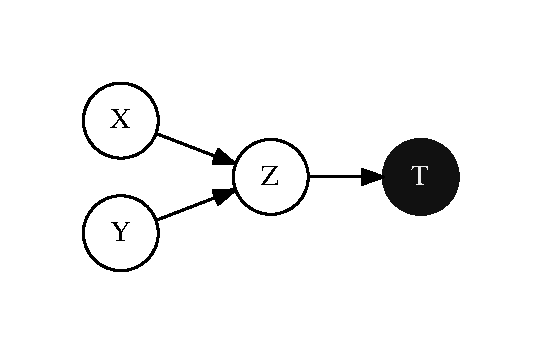
\includegraphics[width=0.5\textwidth]{graph.pdf}
  \caption{Representation of Bayes ball algorithm on Graph G to
    determine if $X$ and $Y$ are conditionally independant given
    $T$}\label{fig:LDA-A-train}
\end{figure}


\end{question}

\begin{question}
  \begin{subquestion}
    Let $(X, Y, Z)$ be random variables on a finite space with $Z$
    binary. Suppose $\indepcond{X}{Y}{Z}$ and $\indep{X}{Y}$.

    If $p(Z = 1) = 0$ or $p(Z = 1) = 1$ we obviously have
    $\indep{X}{Z}$ and $\indep{Y}{Z}$, so we can suppose
    without loss of generality that $p(Z = 1) \ne 0$ and
    $p(Z = 0) \ne 1$.

    To simplify the notation, let us define $\pi$ such that
    \begin{equation*}
      \pi = P(Z = 1)
    \end{equation*}

    We have
    \begin{equation*}
      p(x, y) = \pcond{x, y}{Z = 1} \pi + \pcond{x, y}{Z = 0} (1 - \pi)
    \end{equation*}
    which by hypothesis can be rewriten as
    \begin{equation}
      p(x, y) = \pcond{x}{Z = 1} \pcond{y}{Z = 1} \pi + \pcond{x}{Z = 0} \pcond{y}{Z = 0} (1 - \pi)
      \label{eq:triangle}
      \tag{$\triangle$}
    \end{equation}

    We also have using the second hypothesis :
    \begin{equation*}
        p(x, y) = p(x) p(y) = \left[ \pcond{x}{Z = 1} \pi + \pcond{x}{Z = 0} (1 - \pi) \right]
        \cdot \left[ \pcond{y}{Z = 1} \pi + \pcond{y}{Z = 0} (1 - \pi) \right]
    \end{equation*}

    Developping this expression, we obtain
    \begin{equation*}
      \begin{split}
        p(x, y) & = \pcond{x}{Z = 1} \pcond{y}{Z = 1} \pi^2 \\
        & + \pcond{x}{Z = 0} \pcond{y}{Z = 1} \pi (1 - \pi) \\
        & + \pcond{x}{Z = 1} \pcond{y}{Z = 0} \pi (1 - \pi) \\
        & + \pcond{x}{Z = 0} \pcond{y}{Z = 0} (1 - \pi)^2 \\
      \end{split}
    \end{equation*}

    Since
    \begin{equation*}
      \pi^2 = \pi (\pi - 1) + \pi
    \end{equation*}
    and
    \begin{equation*}
      (1 - \pi)^2 = \pi (\pi - 1) + 1 - \pi
    \end{equation*}

    By replacing in the previous equation,
    \begin{equation*}
      \begin{split}
        p(x, y) & = \pcond{x}{Z = 1} \pcond{y}{Z = 1} (\pi (\pi - 1) + \pi) \\
        & + \pcond{x}{Z = 0} \pcond{y}{Z = 1} \pi (1 - \pi) \\
        & + \pcond{x}{Z = 1} \pcond{y}{Z = 0} \pi (1 - \pi) \\
        & + \pcond{x}{Z = 0} \pcond{y}{Z = 0} ( \pi (\pi - 1) + 1 - \pi) \\
      \end{split}
    \end{equation*}
    Hence,
    \begin{equation*}
      \begin{split}
        p(x, y) & = \pcond{x}{Z = 1} \pcond{y}{Z = 1} \pi + \pcond{x}{Z = 0} \pcond{y}{Z = 0} (1 - \pi) \\
        & - \pcond{x}{Z = 1} \pcond{y}{Z = 1} \pi (1 - \pi) \\
        & + \pcond{x}{Z = 0} \pcond{y}{Z = 1} \pi (1 - \pi) \\
        & + \pcond{x}{Z = 1} \pcond{y}{Z = 0} \pi (1 - \pi) \\
        & - \pcond{x}{Z = 0} \pcond{y}{Z = 0} \pi (1 - \pi) \\
      \end{split}
    \end{equation*}

    By \eqref{eq:triangle}, the first line of the left member is $p(x, y)$, hence
    \begin{equation*}
      \begin{split}
        0 = \pi (1 - \pi) \Big[ &- \pcond{x}{Z = 1} \pcond{y}{Z = 1}  \\
        & + \pcond{x}{Z = 0} \pcond{y}{Z = 1} \\
        & + \pcond{x}{Z = 1} \pcond{y}{Z = 0} \\
        & - \pcond{x}{Z = 0} \pcond{y}{Z = 0} \Big]
      \end{split}
    \end{equation*}
    Which gives
    \begin{equation*}
        \pi (1 - \pi) \left[\pcond{x}{Z = 0} - \pcond{x}{Z = 1} \right] \left[\pcond{y}{Z = 0} - \pcond{y}{Z = 1}\right] = 0
      \end{equation*}

      Since we have supposed that $P(Z = 0) \ne 0$ and
      $P(Z = 1) \ne 0$, we have

      \begin{equation*}
        \pcond{x}{Z = 0} = \pcond{x}{Z = 1} = 0 \text{ or } \pcond{y}{Z = 0} = \pcond{y}{Z = 1}
      \end{equation*}

      \begin{itemize}
      \item If $\pcond{x}{Z = 0} = \pcond{x}{Z = 1}$, then
        \begin{equation*}
          p(x) = \pcond{x}{Z = 0} p(Z = 0) + \pcond{x}{Z = 1} p(Z = 1)
        \end{equation*}
        gives
        \begin{equation*}
          p(x) = \pcond{x}{Z = 0} = \pcond{x}{Z = 1} \\
        \end{equation*}
        Thus,
        \begin{equation*}
          \indep{X}{Z}
        \end{equation*}

      \item else, we have $\pcond{y}{Z = 0} = \pcond{y}{Z = 1}$,
        and we can apply the exact same by symmetry of the variables
        $x$ and $y$,
        \begin{equation*}
          \indep{Y}{Z}
        \end{equation*}


    \end{itemize}

  \end{subquestion}
\end{question}

\section{Distributions factorizing in a graph}

\begin{question}
  The chain rules gives us
  \begin{equation*}
    p(x_i, x_j, x_{\pi_i}) = p(x_{\pi_i}) \pcond{x_i}{x_{\pi_i}} \pcond{x_j}{x_{\pi_i}, x_i}
  \end{equation*}
  and
  \begin{equation*}
    p(x_i, x_j, x_{\pi_i}) = p(x_{\pi_i}) \pcond{x_j}{x_{\pi_i}} \pcond{x_i}{x_{\pi_i}, x_j}
  \end{equation*}
  From that, we deduce that
  \begin{equation}
    \pcond{x_i}{x_{\pi_i}} \pcond{x_j}{x_{\pi_i}, x_i} = \pcond{x_j}{x_{\pi_i}} \pcond{x_i}{x_{\pi_i}, x_j}
    \label{eq:square}
    \tag{$\square$}
  \end{equation}

  Let $\pi_i$ be the set of parents of node $i$ in $G$ and $\rho_i$ be
  the set of parent of $i$ in $G'$.  First we notice that % for every
  % node $k$ different of $i$ and $j$, $\pi_k = \rho_k$
  \begin{equation*}
    \forall k \in \intn{1}{N} \setminus \left\{i, j\right\}, \rho_k = \pi_k
  \end{equation*}
  and we have
  \begin{equation*}
    \rho_i = \pi_i \cup \{j\}
  \end{equation*}
  \begin{equation*}
    \rho_j = \pi_i
  \end{equation*}

  Suppose that p factorizes in $G$, we have

  \begin{equation*}
    p(x) = \prod_{1 \le k \le N} \pcond{x_k}{x_{\pi_k}} =
    \pcond{x_i}{x_{\pi_i}} \pcond{x_j}{x_{\pi_i}, x_i} \prod_{\substack{1 \le k \le N\\
      k \centernot{\in} \left\{i, j\right\}}}
  \pcond{x_k}{x_{\pi_k}}
  \end{equation*}

  By \eqref{eq:square},
  \begin{equation*}
    p(x) =
    \pcond{x_j}{x_{\pi_i}} \pcond{x_i}{x_{\pi_i}, x_j} \prod_{\substack{1 \le k \le N\\
      k \centernot{\in} \left\{i, j\right\}}}
  \pcond{x_k}{x_{\pi_k}}
  \end{equation*}

  Which yields
  \begin{equation*}
    p(x) =
    \pcond{x_j}{x_{\rho_j}} \pcond{x_i}{x_{\rho_i}} \prod_{\substack{1 \le k \le N\\
        k \centernot{\in} \left\{i, j\right\}}}
    \pcond{x_k}{x_{\rho_k}} =
    \prod_{1 \le k \le N} \pcond{x_k}{x_{\rho_k}}
  \end{equation*}

  This proves that $\mathcal{L}(G) \subset \mathcal{L}(G')$. By applying
  the same operation on the graph $G'$ with the covered edge $(j, i)$,
  we obtain that $\mathcal{L}(G') \subset \mathcal{L}(G)$

  Hence $\mathcal{L}(G) = \mathcal{L}(G')$

\end{question}

\begin{question}
  We start by a lemma,
  \begin{lemma}
    The maximum cardinal of a clique in an undirected tree is $2$
  \end{lemma}

  \begin{proof}
    If we had a clique of cardinal $n > 2,\ x_0, x_1, \dots x_n$, by
    definition of the clique, $(x_0, x_1, x_2)$ and $(x_0, x_2)$ would
    be two distinct path from $x_0$ to $x_2$. By definition, of an
    undirected tree, two vertices are connected by exactly one path,
    hence the contradiction.
  \end{proof}

  Let $p \in \mathcal{L}(G)$, then we have
  \begin{equation*}
    p(x) = \prod_{i = 1}^N \pcond{x_i}{x_{\pi_i}}
  \end{equation*}

  Based on the lemma, if we index $G$ with a topological order
  (starting from $0$ for the root, to $n$) and $G'$ with the same
  indices, the cliques of cardinal 2 in $G'$ form the set
  $\set{(x_i, x_{\pi_i})}{1 \le i \le n}$ where $x_{\pi_i}$ is the set
  of parent of the node $x_i$ (it contains at most one element). the
  cliques of cardinal 1 are obviously defined by the set of nodes
  $\set{x_i}{0 \le i \le n}$.

  Therefore, we can write
  \begin{equation*}
    p(x) = \prod_{i = 0}^N \phi_i(x_i, x_{\pi_i})
  \end{equation*}

  or equivalently

  \begin{equation*}
    p(x) = \prod_{C \in \mathcal{C}} \phi_C(x_C)
  \end{equation*}

  % Where $\phi_C = \pcond{x_i}{x_{pi_i}}$ if $C = (x_i, x_{\pi_i})$
  % and $\phi_C = p(x_i)$ if $C = (x_i)$

  with

  \begin{equation*}
    \phi_C = \left\{
      \begin{array}{lll}
        \pcond{x_i}{x_{\pi_i}} &\text{ if } C = (x_i, x_{\pi_i}) \\
        p(x_i) &\text{ if } C = (x_i) \text{ and } x_{\pi_i} = \varnothing \\
        1 &\text{ if } C = (x_i) \text{ and } x_{\pi_i} \ne \varnothing \\
      \end{array}
    \right.
  \end{equation*}

  Hence $p \in \mathcal{L}(G)$.

  Suppose now that $p \in \mathcal{L}(G')$. By the previous
  reasonement on the cliques of an undirected tree, and using the same
  indexing as before we can write
  \begin{equation*}
    p(x) = \prod_{i = 0}^N \phi_i(x_i, x_{\pi_i})
  \end{equation*}

  % Let us show by recurrence that
  % \begin{equation*}
  %   p(x) = \prod_{i = 0}^N \pcond{x_i}{x_{\pi_i}}
  % \end{equation*}

  % This is






\end{question}



\section{Entropy and Mutual Information}

\begin{question}
  Let X be a discrete random variable on $\mathcal{X}$. Let
  $p_X(x)$ denote its probability mass function.

  \begin{subquestion}
    For all $x \in \mathcal{X}$, $0 \le p_X(x) \le 1$, hence
    \begin{equation*}
      \forall x \in \mathcal{X}, - \log{p_X(x)} \ge 0
    \end{equation*}
    Hence,
    \begin{equation*}
      \forall x \in \mathcal{X}, - p_X(x)\log{p_X(x)} \ge 0
    \end{equation*}
    Summing over the set $\mathcal{X}$ we obtain that $H(X) \ge 0$.

    Let us prove that $H(X) = 0$ if and only if X is a constant with
    probability 1.

    \ipart{Necessary condition}

    if X is constant with probability 1,
    \begin{equation*}
      \exists c \in \mathcal{X}, \left\{
        \begin{array}{l}
          p_X(c) = 1 \\
          \forall x \ne c, p_X(x) = 0  \\
        \end{array}
      \right.
    \end{equation*}
    Hence each term of the sum in the entropy is null
    \begin{equation*}
      \forall x \in \mathcal{X},\ p_X(x) \log{p_X(x)} = 0\\
    \end{equation*}
    And
    \begin{equation*}
      H(X) = \sum_{x \in \mathcal{X}} p_X(x) \log{p_X(x)} = 0\\
    \end{equation*}
    % Let us consider such a $c$.
    % \begin{equation*}
    %   \forall x \ne c, p_X(x)\log{p_X(x)} = 0
    % \end{equation*}
    % and $p_X(c) = 0$
    % Hence

    \ipart{Sufficient condition}

    Suppose $H(X) = 0$.

    H is a sum of positive terms. If there were a $\tilde{x} \in \mathcal{X}$,
    such that $0 < p_X(\tilde{x}) < 1$, then we would have
    $-p_X(\tilde{x}) \log{p_X(\tilde{x})} > 0$, hence

    \begin{equation*}
      -\sum_{x \in \mathcal{X}} p_X(x) \log{p_X(x)} \ge -p_X(\tilde{x}) \log{p_X(\tilde{x})} > 0
    \end{equation*}

    (One of the term of H(X) would be strictly positive and H would be
    strictly positive)

    We deduce that
    \begin{equation*}
      \forall x \in \mathcal{X},\ p_X(x) = 0 \text{ or } p_X(x) = 1
      \label{eq:circle1}
      \tag{$\Diamond_1$}
    \end{equation*}
    % for H to be zero, we must have

    % \begin{equation*}
    %   \forall x \in \mathcal{X},\ p_X(x) \log{p_X(x)} = 0
    % \end{equation*}

    % \begin{align*}
    %   H(X) = 0 & \iff -\sum_{x \in \mathcal{X}} p_X(x) \log{p_X(x)} = 0 \\
    %   & \iff \forall x \in \mathcal{X},\ p_X(x) \log{p_X(x)} = 0
    % \end{align*}

    % \begin{equation*}
    %   H(X) = 0 \iff \forall x \in \mathcal{X},\ \left\{
    %     \begin{array}{ll}
    %       p_X(x) \log{p_X(x)} = 0
    %     \end{array}
    %   \right.
    % \end{equation*}

    Moreover by definition,
    \begin{equation*}
      \sum_{x \in \mathcal{X}} p_X(x) = 1
      \label{eq:circle2}
      \tag{$\Diamond_2$}
    \end{equation*}

    In order to satisfy both \eqref{eq:circle1} and \eqref{eq:circle2},
    we must have exactly one $c \in \mathcal{X}$ such that $p_X(c) = 1$ and
    $\forall x \in \mathcal{X} \setminus \{c\},\ p_X(x) = 0$, which means
    that X is constant with probability 1.
  \end{subquestion}

  \begin{subquestion}
    We have $\forall x \in \mathcal{X} q(x) = \frac{1}{k}$, and the
    Kullback-Leibler divergence between p and q is finite.

    We can write
    \begin{equation*}
      \kldiv{p}{q} = \sum_{x \in \mathcal{X}}p(x) \log(p(x)) - \sum_{x \in \mathcal{X}}p(x) \log\left(\frac{1}{k}\right)
    \end{equation*}

    Hence,
    \begin{equation*}
      \kldiv{p}{q} = -H(X) + \log\left(k\right)
    \end{equation*}

  \end{subquestion}

  \begin{subquestion}
    Since we know that $\kldiv{p}{q} \ge 0$, we obtain immediately

    \begin{equation*}
      H(X) \le \log\left(k\right)
    \end{equation*}

    We note that the upper bound on the entropy is the entropy of
    a random variable uniformely distributed over $\mathcal{X}$.

    \begin{equation*}
      H(Y) = -\sum_{x \in \mathcal{X}} \frac{1}{k} \log\left(\frac{1}{k}\right) = \log\left(k\right)
    \end{equation*}


  \end{subquestion}


\end{question}

\begin{question}
  Let $(X_1, X_2)$ a pair of discrete random variables defined over
  $\mathcal{X}_1 \times \mathcal{X}_2$.
  \begin{subquestion}
    We have
    \begin{equation*}
      I(X_1, X_2) = \sum_{x_1 \in \mathcal{X}_1} \sum_{x_2 \in \mathcal{X}_2} p(x_1, x_2) \log{\dfrac{p(x_1, x_2)}{p(x_1) p(x_2)}}
    \end{equation*}

    % If $\exists (x_1, x_2) \in \mathcal{X}_1 \times \mathcal{X}_2 ,\ p(x_1) = 0$ and $p(x_1, x_2) > 0$, $I(X_1, X_2) = + \infty$

    This can be rewriten as
    \begin{equation*}
      I(X_1, X_2) = \sum_{x_1 \in \mathcal{X}_1} \sum_{x_2 \in \mathcal{X}_2} p(x_1) p(x_2) \dfrac{p(x_1, x_2)}{p(x_1) p(x_2)} \log{\dfrac{p(x_1, x_2)}{p(x_1) p(x_2)}}
    \end{equation*}

    Let $f$ be the function
    \begin{equation*}
      \begin{array}{lll}
        \mathbb{R}^+ & \to & \mathbb{R} \\
        x & \mapsto & x \log{x}
      \end{array}
    \end{equation*}
    This function is convex (twice differentiable, with $f''(x) = 1 / x$), and since
    \begin{equation*}
      \sum_{x_1 \in \mathcal{X}_1} \sum_{x_2 \in \mathcal{X}_2} p(x_1) p(x_2) = \left( \sum_{x_1 \in \mathcal{X}_1} p(x_1) \right) \left( \sum_{x_2 \in \mathcal{X}_2} p(x_2) \right) = 1
    \end{equation*}
    Jensen inequality gives us
    \begin{equation*}
      f\left(\sum_{x_1 \in \mathcal{X}_1} \sum_{x_2 \in \mathcal{X}_2} p(x_1) p(x_2) \dfrac{p(x_1, x_2)}{p(x_1) p(x_2)}\right) \le \sum_{x_1 \in \mathcal{X}_1} \sum_{x_2 \in \mathcal{X}_2} p(x_1) p(x_2) f\left(\dfrac{p(x_1, x_2)}{p(x_1) p(x_2)}\right)
    \end{equation*}

    Since
    \begin{equation*}
      f\left(\sum_{x_1 \in \mathcal{X}_1} \sum_{x_2 \in \mathcal{X}_2} p(x_1) p(x_2) \dfrac{p(x_1, x_2)}{p(x_1) p(x_2)}\right) = f\left(\sum_{x_1 \in \mathcal{X}_1} \sum_{x_2 \in \mathcal{X}_2} p(x_1, x_2)\right) = f(1) = 0
    \end{equation*}

    And
    \begin{equation*}
      \sum_{x_1 \in \mathcal{X}_1} \sum_{x_2 \in \mathcal{X}_2} p(x_1) p(x_2) f\left(\dfrac{p(x_1, x_2)}{p(x_1) p(x_2)}\right)
      % = \sum_{x_1 \in \mathcal{X}_1} \sum_{x_2 \in \mathcal{X}_2} p(x_1) p(x_2) \dfrac{p(x_1, x_2)}{p(x_1) p(x_2)} \log{\dfrac{p(x_1, x_2)}{p(x_1) p(x_2)}}
      = I(X_1, X_2)
    \end{equation*}

    We obtain
    \begin{equation*}
      I(X_1, X_2) \ge 0
    \end{equation*}

  \end{subquestion}

  \begin{subquestion}

    We can rewrite the mutual information as
    \begin{equation*}
      \begin{split}
        I(X_1, X_2)
        = & \sum_{x_1 \in \mathcal{X}_1} \sum_{x_2 \in \mathcal{X}_2} p(x_1, x_2) \log{\Bigl(p(x_1, x_2)\Bigr)} \\
        & - \sum_{x_1 \in \mathcal{X}_1} \sum_{x_2 \in \mathcal{X}_2} p(x_1, x_2) \log{\Bigl(p(x_1)\Bigr)} \\
        & - \sum_{x_1 \in \mathcal{X}_1} \sum_{x_2 \in \mathcal{X}_2} p(x_1, x_2) \log{\Bigl(p(x_2)\Bigr)}
      \end{split}
    \end{equation*}

    We can simplify
    \begin{equation*}
      \begin{split}
        I(X_1, X_2)
        = & \sum_{x_1 \in \mathcal{X}_1} \sum_{x_2 \in \mathcal{X}_2} p(x_1, x_2) \log{\Bigl(p(x_1, x_2)\Bigr)} \\
        & - \sum_{x_1 \in \mathcal{X}_1} \left(\sum_{x_2 \in \mathcal{X}_2} p(x_1, x_2)\right) \log{\Bigl(p(x_1)\Bigr)} \\
        & - \sum_{x_2 \in \mathcal{X}_2} \left(\sum_{x_1 \in \mathcal{X}_1} p(x_1, x_2)\right) \log{\Bigl(p(x_2)\Bigr)}
      \end{split}
    \end{equation*}

    Hence,
    \begin{equation*}
      \begin{split}
        I(X_1, X_2)
        = & \sum_{x_1 \in \mathcal{X}_1} \sum_{x_2 \in \mathcal{X}_2} p(x_1, x_2) \log{\Bigl(p(x_1, x_2)\Bigr)} \\
        & - \sum_{x_1 \in \mathcal{X}_1} p(x_1) \log{\Bigl(p(x_1)\Bigr)} \\
        & - \sum_{x_2 \in \mathcal{X}_2} p(x_2) \log{\Bigl(p(x_2)\Bigr)}
      \end{split}
    \end{equation*}

    % \begin{equation*}
    %   \sum_{x_1 \in \mathcal{X}_1} \sum_{x_2 \in \mathcal{X}_2} p(x_1, x_2) \log{\Bigl(p(x_1)\Bigr)}
    %   = \sum_{x_1 \in \mathcal{X}_1} \left(\sum_{x_2 \in \mathcal{X}_2} p(x_1, x_2) \right) \log{\Bigl(p(x_1)\Bigr)}
    %   = \sum_{x_1 \in \mathcal{X}_1} p(x_1) \log{\Bigl(p(x_1)\Bigr)}
    %   = H(X_1)
    % \end{equation*}

    % Similarly,
    % \begin{equation*}
    %   \sum_{x_1 \in \mathcal{X}_1} \sum_{x_2 \in \mathcal{X}_2} p(x_1, x_2) \log{\Bigl(p(x_2)\Bigr)}
    %   % = \sum_{x_2 \in \mathcal{X}_2} p(x_2) \log{\Bigl(p(x_2)\Bigr)}
    %   = H(X_2)
    % \end{equation*}

    If we consider the variable $X = (X_1, X_2)$, we can write its entropy as
    \begin{align*}
      H(X)
      & = - \sum_{x \in \mathcal{X}_1 \times \mathcal{X}_2} p_X(x)\log{p_X(x)} \\
      % & = - \sum_{x_1 \in \mathcal{X}_1} \sum_{x_2 \in \mathcal{X}_2} p_{1,2}(x_1, x_2)\log{p_X(x_1, x_2)} \\
      & = - \sum_{x \in \mathcal{X}_1 \times \mathcal{X}_2} p(x_1, x_2) \log{\Bigl(p(x_1, x_2)\Bigr)}
    \end{align*}

    Hence,
    \begin{equation*}
      I(X_1, X_2) = - H(X_1, X_2) + H(X_1) + H(X_2)
    \end{equation*}

    % \begin{align*}
    %   I(X_1, X_2)
    %   & = \sum_{x_1 \in \mathcal{X}_1} \sum_{x_2 \in \mathcal{X}_2} p(x_1, x_2) \log{\dfrac{p(x_1, x_2)}{p(x_1) p(x_2)}} \\
    %   & = \sum_{x_1 \in \mathcal{X}_1} \sum_{x_2 \in \mathcal{X}_2} p(x_1, x_2) \log{\Bigl(p(x_1, x_2)\Bigr)} - \sum_{x_1 \in \mathcal{X}_1} \sum_{x_2 \in \mathcal{X}_2} p(x_1, x_2) \log{\Bigl(p(x_1)p(x_2)\Bigr)} \\
    %   & = \sum_{x_1 \in \mathcal{X}_1} \sum_{x_2 \in \mathcal{X}_2} p(x_1, x_2) \log{\Bigl(p(x_1, x_2)\Bigr)} - \sum_{x_1 \in \mathcal{X}_1} \sum_{x_2 \in \mathcal{X}_2} p(x_1, x_2) \log{\Bigl(p(x_1)\Bigr)} - \sum_{x_1 \in \mathcal{X}_1} \sum_{x_2 \in \mathcal{X}_2} p(x_1, x_2) \log{\Bigl(p(x_2)\Bigr)} \\
    % \end{align*}

  \end{subquestion}

  \begin{subquestion}
    From the two previous question,
    we have
    \begin{equation*}
      I(X_1, X_2) = - H(X_1, X_2) + H(X_1) + H(X_2) \ge 0
    \end{equation*}
    e.g.
    \begin{equation*}
      H(X_1, X_2) \le H(X_1) + H(X_2)
    \end{equation*}

    And if we note $p$ the joint probablity distribution that make
    $X_1$ and $X_2$ independent, and $X$ the random
    variable associated with this probability distribution, e.g.
    % TODO verify that it actually means something
    \begin{equation*}
      \forall (x_1, x_2) \in \mathcal{X}_1 \times \mathcal{X}_2,\ p(x_1, x_2) = p(x_1) p(x_2)
    \end{equation*}

    \begin{align*}
      H(X) & = - \sum_{x \in \mathcal{X}_1 \times \mathcal{X}_2 } p(x_1, x_2) \log{\Bigl( p(x_1, x_2) \Bigr)} \\
           & = - \sum_{x \in \mathcal{X}_1 \times \mathcal{X}_2 } p(x_1) p(x_2) \log{\Bigl( p(x_1) \Bigr)}
             - \sum_{x \in \mathcal{X}_1 \times \mathcal{X}_2 } p(x_1) p(x_2) \log{\Bigl( p(x_2) \Bigr)} \\
           & = - \sum_{x_1 \in \mathcal{X}_1 } p(x_1) \log{\Bigl( p(x_1) \Bigr)}
             - \sum_{x_2 \in \mathcal{X}_2 } p(x_2) \log{\Bigl( p(x_2) \Bigr)} \\
           & = H(X_1) + H(X_2)
    \end{align*}

    Which means that the maximum entropy is obtained when $X_1$ and $X_2$
    are independant.
    % TODO comment more ?

  \end{subquestion}

\end{question}

\section{Implementation - Gaussian mixtures}

\begin{subquestion}
  The file \emph{clustering.py} contains my implementation in python of
  the \emph{K-means} algorithm. It uses random points as initialization.
  I used a function that I found online to show the voronoi cells in the
  case of K-means.

  For $K=4$, the algorithm seems to almost always converge to the same
  local optimum ($3237.8$ distortion), I ran the algorithm $5000$
  times and plotted the histogram representing the number of
  iterations to convergence \figref{fig:kmeans4-iterations-hist} and
  the histogram representing the distortion
  \figref{fig:kmeans4-distortion-hist} In the distortion histogram,
  the second bar represents ($29$ run of the algorithm over $5000$,
  which means that the algorithm has converged to the global optimum
  $99.42\%$ of the $5000$ runs)

  \begin{figure}[h!]
    \centering
    \begin{subfigure}[t]{0.48\textwidth}
      \centering
      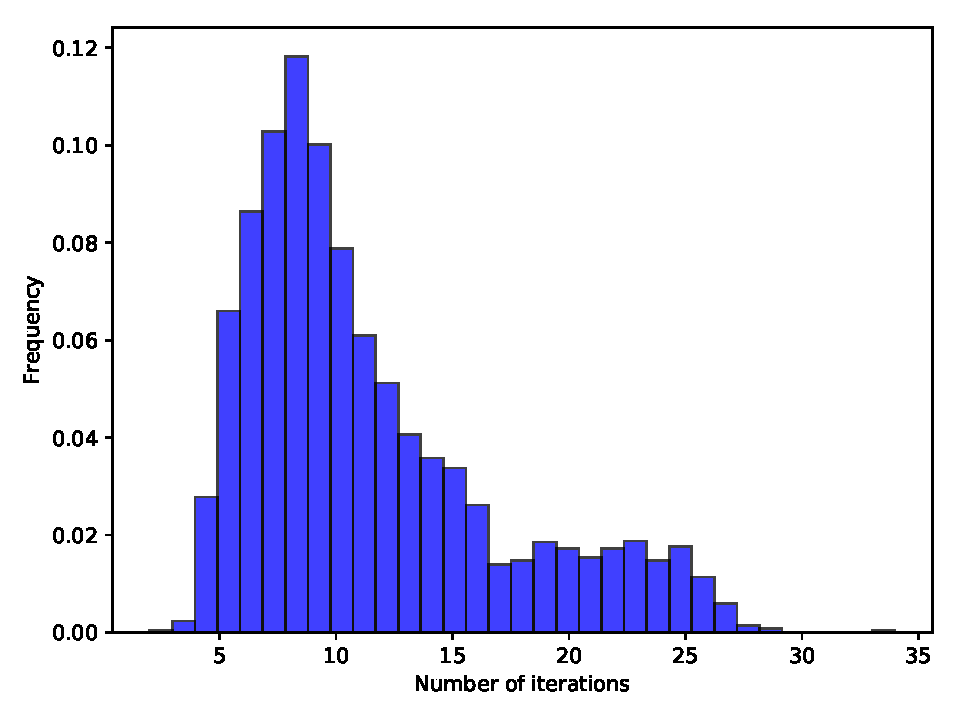
\includegraphics[width=\textwidth]{kmeans4_iterations_hist.pdf}
      \caption{Histogram of the number of iterations}\label{fig:kmeans4-iterations-hist}
    \end{subfigure}
    \quad
    \begin{subfigure}[t]{0.48\textwidth}
      \centering
      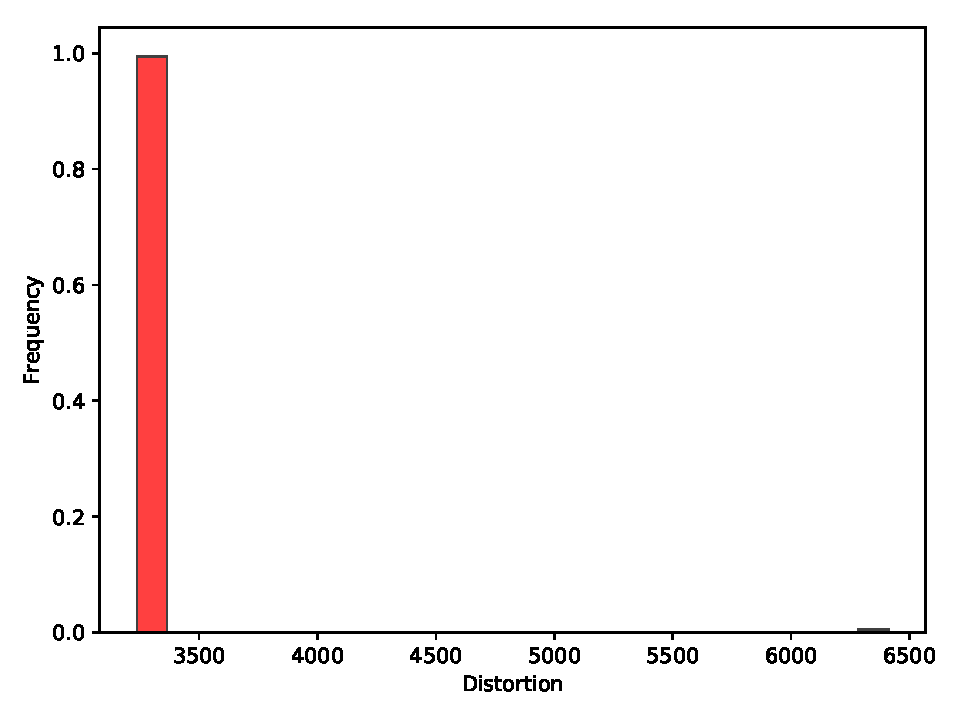
\includegraphics[width=\textwidth]{kmeans4_distortion_hist.pdf}
      \caption{Histogram of the distortion}\label{fig:kmeans4-distortion-hist}
    \end{subfigure}
    \caption{Histogram representing the number of iterations and the
      distortion for $5000$ iterations of the algorithm K-means with
      $K=4$ on the training data}\label{fig:kmeans4-hist}
  \end{figure}

  The result obtained $99.42\%$ of the runs by the algorithm is
  presented in figure \ref{fig:kmeans4-success}, and the evolution of
  distortion is given in figure \ref{fig:kmeans4-distortion}. Since
  the histogram of the distortion presents cases where the algorithm
  converges to a worst local optimum, I managed to find one such
  example, it's presented in the figure \ref{fig:kmeans4-failure}
  (this K-means execution resulted in a distortion of $6378.84$ and
  converged in $5$ steps)

  \begin{figure}[h!]
    \centering
    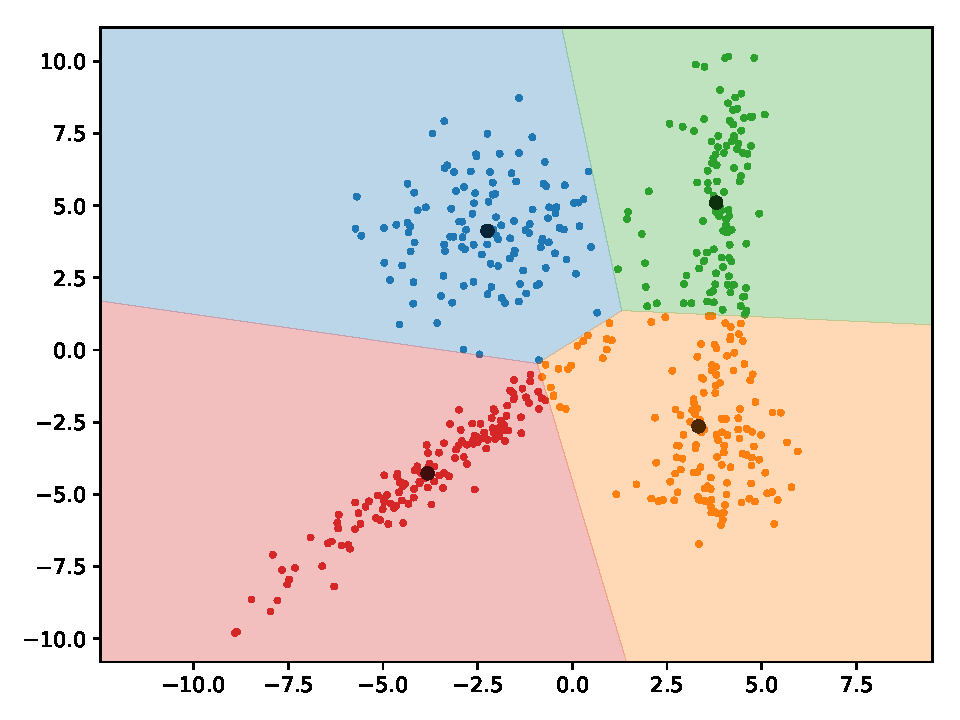
\includegraphics[width=0.7\textwidth]{kmeans4_success.pdf}
    \caption{Representation of the training points, the means returned
      by an execution of the K-means algorithm ($K = 4$) (and
      the Voronoi partition of the space associated) (distortion =
      3237.78, convergence in 7
      iterations)}\label{fig:kmeans4-success}
  \end{figure}

  \begin{figure}[h!]
    \centering
    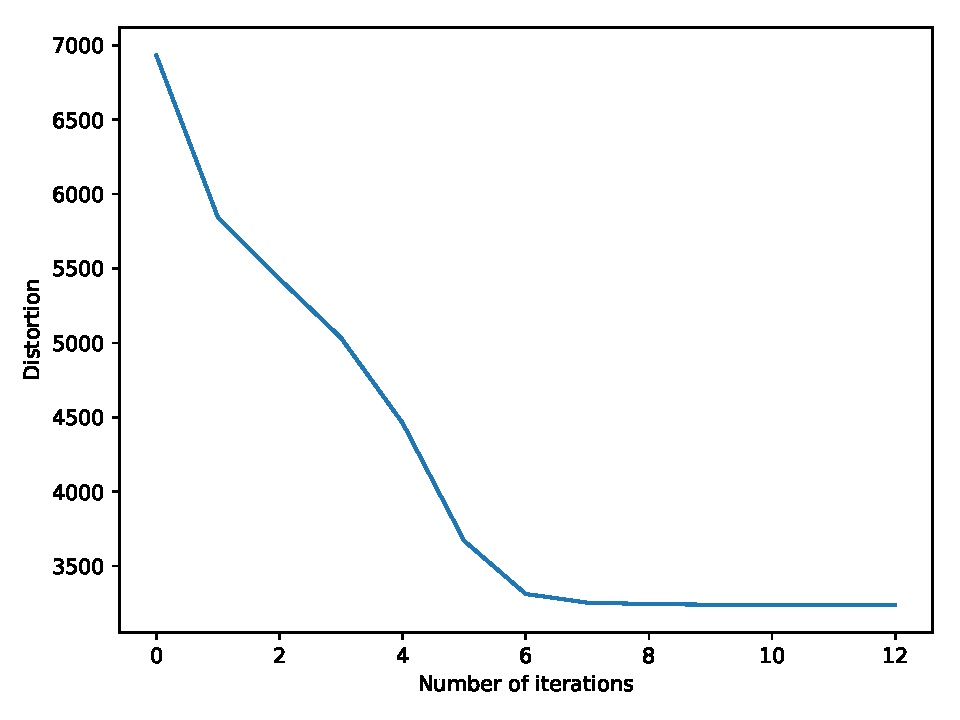
\includegraphics[width=0.6\textwidth]{kmeans4_distortion.pdf}
    \caption{Evolution of the distortion with respect to the number of
      iterations for an execution of the Kmeans algorithm}\label{fig:kmeans4-distortion}
  \end{figure}

  \begin{figure}[h!]
    \centering
    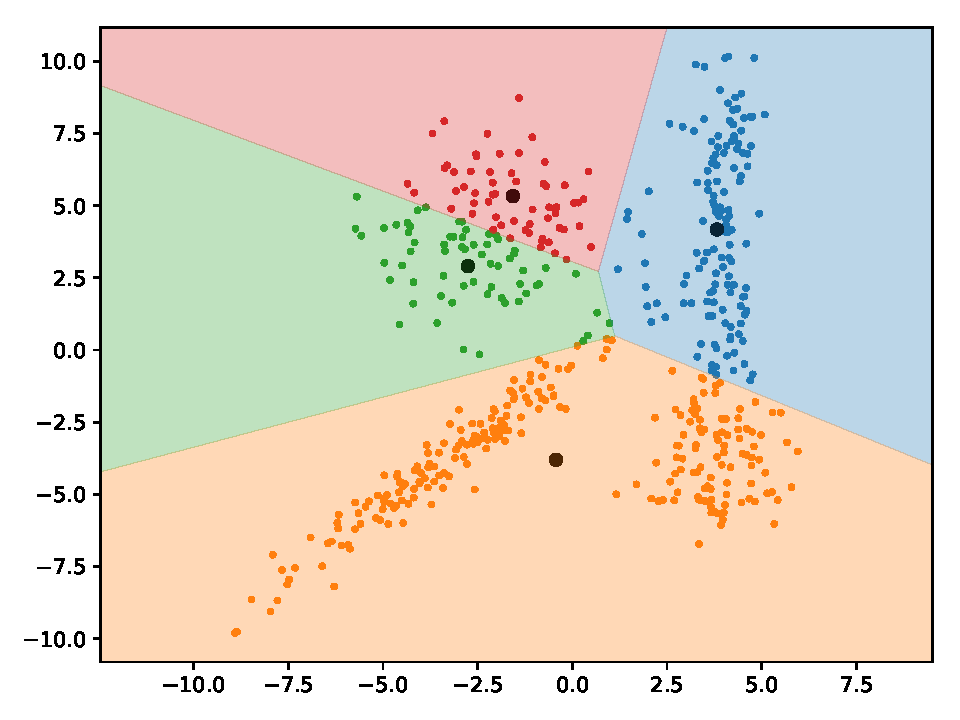
\includegraphics[width=0.7\textwidth]{kmeans4_failure.pdf}
    \caption{Representation of the training points, the means returned
      by an execution of the K-means algorithm ($K = 4$) that has
      converged to a bad local minimum (distortion =
      6378.84, convergence in 5
      iterations)}\label{fig:kmeans4-failure}
  \end{figure}




  % one case : distortion 6378.83747556 n_iter = 5




  % The results of the distortion and the number of iteration for 10 runs of the algorithms are
  % given in the table~\ref{tab:kmeans-4-10}

  % \begin{table}[h!]
  %   \centering
  %   \begin{tabular}{|l|c|c|c|c|c|}
  %     \hline
  %     Distortion & 3240.59 & 3240.17 & 3238.14 & 3240.17 & 3240.17 \\
  %     \hline
  %     Iterations & 11 & 4 & 6 & 24 & 25 \\

  %     \hline\hline

  %     Distortion & 3237.67 & 3240.17 & 3238.69 & 3237.67 & 3240.17 \\
  %     \hline
  %     Iterations & 13 & 23 & 11 & 8 & 10 \\
  %     \hline
  %   \end{tabular}
  %   \captionof{table}{Representation of the distortion and the number
  %     of iteration for 10 runs of the K-mean algorithm with random
  %     start for $K=4$ } \label{tab:kmeans-4-10}
  % \end{table}

\end{subquestion}

\newpage
\begin{subquestion}
  Let's rewrite the EM algorithm under the hypothesis
  \begin{equation*}
    \forall k \in \intn{1}{K}, \Sigma_k = \sigma_k^2 \cdot \text{Id}_d
  \end{equation*}
  we have
  \begin{equation*}
    \forall k \in \intn{1}{K}, \det{\Sigma_k} = \sigma_k^{2d}
  \end{equation*}

  \ipart{E step}

  The probability $\parampcond{\theta}{z_i = j}{x_i}$ is
  \begin{equation*}
    \parampcond{\theta}{z_i = j}{x_i} =
    \dfrac
    {\frac{\pi_j}{\sigma_j^d} \exp{ \left( -\dfrac{\norm{x_i - \mu_j}^2}{2 \sigma_j^2} \right)}}
    {\bigsum_{k = 1}^K \frac{\pi_k}{\sigma_k^d} \exp{ \left( -\dfrac{\norm{x_i - \mu_k}^2}{2 \sigma_k^2} \right)}}
    = \tau_i^j
  \end{equation*}

  The complete log likelihood is given by
  \begin{equation*}
    \begin{split}
      \log{p_\theta (x, z)}
      & = \sum_{i = 1}^N \sum_{j = 1}^K z_i^j \log{\pi_j} \\
      & - \dfrac{d N}{2} \log{2 \pi} - \dfrac{d}{2} \sum_{i = 1}^N \sum_{j = 1}^K z_i^j \log{\sigma_j^2} \\
      & - \dfrac{1}{2} \sum_{i = 1}^N \sum_{j = 1}^K z_i^j \dfrac{\norm{x_i - \mu_j}^2}{\sigma_j^2}
    \end{split}
  \end{equation*}


  As explained in the lesson, taking the expectation with respect to
  the conditionnal distribution of Z given X is equivalent to replacing
  $z_i^j$ by
  \begin{equation*}
    E_{Z | X}[z_i^j] = 0 \cdot \pcond{z_i^j = 0}{x} + 1 \cdot \pcond{z_i^j = 1}{x} = \pcond{z_i = j}{x_i}
  \end{equation*}

  Hence,
  \begin{equation*}
    \begin{split}
      E_{Z | X}[\log{p_\theta (x, z)}]
      &=\sum_{i = 1}^N \sum_{j = 1}^K  \parampcond{\theta}{z_i = j}{x_i} \log{\pi_j} \\
      & - \dfrac{d N}{2} \log{2 \pi} - \dfrac{d}{2} \sum_{i = 1}^N \sum_{j = 1}^K \parampcond{\theta}{z_i = j}{x_i} \log{\sigma_j^2} \\
      & - \sum_{i = 1}^N \sum_{j = 1}^K \parampcond{\theta}{z_i = j}{x_i} \dfrac{\norm{x_i - \mu_j}^2}{2 \sigma_j^2}
    \end{split}
  \end{equation*}

  Which by replacing the expression of $\parampcond{\theta}{z_i = j}{x_i}$, gives
  \begin{equation}
    \label{eq:expected-complete-likelihood}
    \tag{$ECL$}
    \begin{split}
      E_{Z | X}[\log{p_\theta (x, z)}]
      &=\sum_{i = 1}^N \sum_{j = 1}^K  \tau_i^j(\theta) \log{\pi_j} \\
      & - \dfrac{d N}{2} \log{2 \pi} - \dfrac{d}{2} \sum_{i = 1}^N \sum_{j = 1}^K \tau_i^j \log{\sigma_j^2} \\
      & - \sum_{i = 1}^N \sum_{j = 1}^K \tau_i^j(\theta) \dfrac{\norm{x_i - \mu_j}^2}{2 \sigma_j^2}
    \end{split}
  \end{equation}

  \ipart{M step}

  In this sum, we can maximize separately over $\pi$ and
  $(\mu, \sigma^2)$, because the expression of the expected complete
  log-likelihood is a sum of a function which only depends on $\pi$
  and a function which only depends on $(\mu, \sigma^2)$

  \ipart{Maximizing over $\pi$}

  We have the following problem
  \begin{equation*}
    \begin{aligned}
      & \underset{\pi}{\text{maximize}}
      & & \sum_{i = 1}^N\sum_{j = 1}^K\tau_i^j \log{\pi_j} \\
      & \text{subject to}
      & & \pi_1 + \dots + \pi_K = 1
    \end{aligned}
  \end{equation*}

  This is a convex problem, with affine constraints, it's feasible,
  hence by slater's constraint, strong duality holds. If we derive
  \wrt $\pi_k$ the following
  \begin{equation*}
    \sum_{i = 1}^N\sum_{j = 1}^K\tau_i^j \log{\pi_j} + \lambda \left(\sum_{j = 1}^K\pi_j - 1\right)
  \end{equation*}
  we obtain
  \begin{equation*}
    \sum_{i = 1}^N \dfrac{\tau_i^k}{\pi_k} + \lambda = 0
  \end{equation*}
  If we let $\hat{\pi}$ such that
  \begin{equation*}
    \forall k \in \intn{1}{K},\ \hat{\pi}_k = \dfrac{\sum_{i = 1}^N \tau_i^k}{\sum_{i = 1}^N\sum_{j = 1}^K\tau_i^j}
  \end{equation*}
  and
  \begin{equation*}
    \hat{\lambda} = \sum_{i = 1}^N\sum_{j = 1}^K\tau_i^j
  \end{equation*}
  Then, $(\hat{\pi}, \hat{\lambda})$ statisfy the K.K.T conditions, hence $\hat{\pi}$ is
  the primal solution of the problem.

  \ipart{Maximizing over $\mu$}

  The expected complete likelihood function is concave \wrt
  $(\mu, \sigma^2)$ (not strictly) (the hessian has 2 non zero
  eigenvalues which are negative).

  The gradient of the expected complete likelihood \wrt to $\mu_k$
  is zero when
  \begin{equation*}
    \sum_{i = 1}^N\tau_i^k \dfrac{(x_i - \hat{\mu}_k)}{2 \sigma_k^2} = 0 \iff \hat{\mu}_k = \dfrac{\sum_{i = 1}^N\tau_i^k x_i}{\sum_{i = 1}^N\tau_i^k}
  \end{equation*}

  \ipart{Maximizing over $\sigma^2$}

  The gradient of the expected complete likelihood \wrt to $\sigma_k^2$
  is zero when
  \begin{align*}
    - \dfrac{d}{2} \sum_{i = 1}^N\dfrac{\tau_i^k}{\hat{\sigma}_k^2} + \dfrac{1}{2} \sum_{i = 1}^N \tau_i^k \dfrac{\norm{x_i - \mu_k}^2}{\hat{\sigma}_k^4} = 0
    & \iff - d \sum_{i = 1}^N \tau_i^k + \sum_{i = 1}^N \tau_i^k \dfrac{\norm{x_i - \mu_k}^2}{\hat{\sigma}_k^2} = 0 \\
    & \iff \hat{\sigma}_k^2 = \dfrac{\sum_{i = 1}^N \tau_i^k \norm{x_i - \mu_k}^2}{d \sum_{i = 1}^N \tau_i^k} \\
  \end{align*}

  \ipart{Results}

  The figure \ref{fig:sphericalEM4-success} represents an execution of
  the algorithm. The points of the training data are represented in
  the color of the most probable value of their corresponding latent
  variable. For each gaussian distribution, the mean is represented in
  black, the ellipse containing 90\% of the distribution is also
  represented. The evolution of the likelihood with respect to the
  number of iteration is given in figure
  \ref{fig:sphericalEM4-likelihood}.

  \begin{figure}[h!]
    \centering
    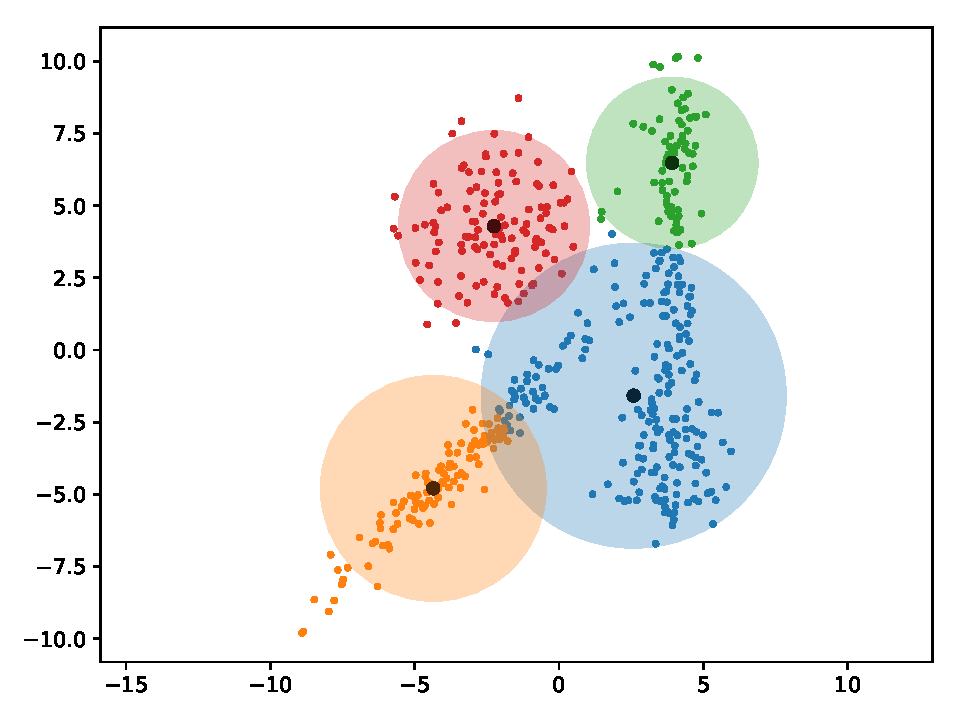
\includegraphics[width=0.7\textwidth]{sphericalEM4_success.pdf}
    \caption{Representation of the training points, the means returned
      by anw execution of the spherical EM algorithm ($K = 4$). the
      disks represented contain 90\% of the mass of the associated
      gaussian distribution (likelihood is $-2645.53$, convergence in $71$
      iterations, for $\epsilon = 10^{-6}$)}\label{fig:sphericalEM4-success}
    % incomplete likelihood -2645.52636142
  \end{figure}

  \begin{figure}[h!]
    \centering
    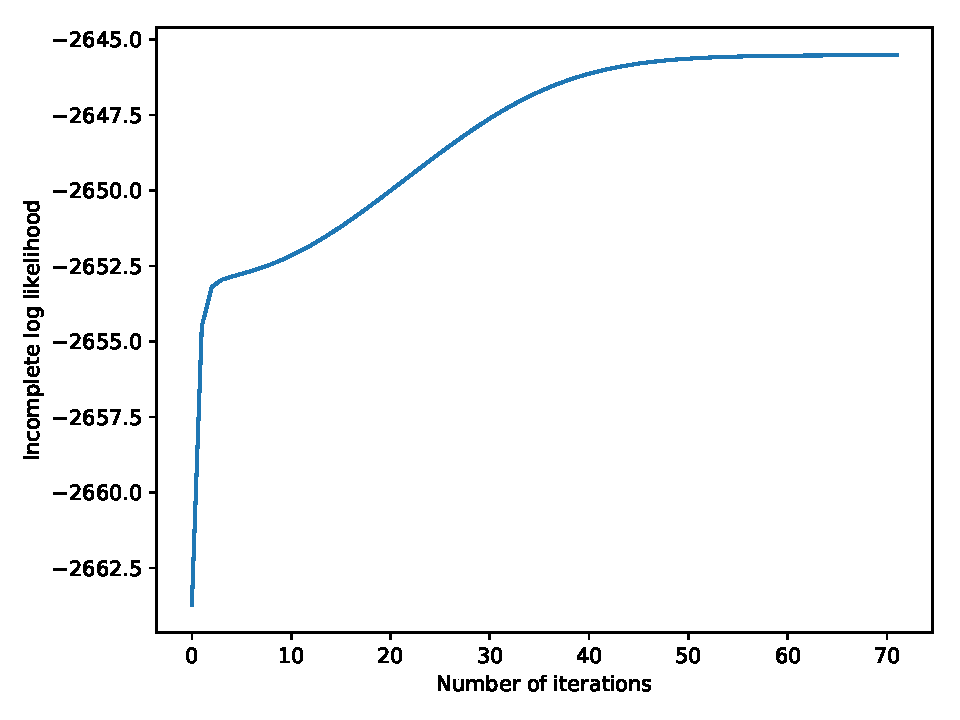
\includegraphics[width=0.6\textwidth]{sphericalEM4_likelihood.pdf}
    \caption{Evolution of the incomplete log likelihood with respect
      to the number of iterations for an execution of the EM algorithm
      for gaussian mixture with isotropic
      covariance}\label{fig:sphericalEM4-likelihood}
  \end{figure}


  The algorithm stops when the absolute difference of the incomplete
  likelihood is less than a given threshold $\epsilon$ from one
  iteration to the next. (I divide by the number of point so that the
  threshold does not depends on the number of point, and also because
  the threshold in \emph{scikit-learn} corresponds exactly to this
  quantity, which makes it possible to compare speed for a given
  threshold (see in conclusion))

  I've run $5000$ iteration of the algorithm on training sample, and
  plotted the histogram representing the number of iteration and the
  estimated complete likelihood it has converged to
  \figref{fig:sphericalEM4-hist}).  By looking at the histogram, we
  can see that there are cases where the algorithm sometimes converges
  to a local minimum that is \say{far} from the optimum, figure
  \ref{fig:sphericalEM4-failure} represents one such case

  \begin{figure}[h!]
    \centering
    \begin{subfigure}[t]{0.48\textwidth}
      \centering
      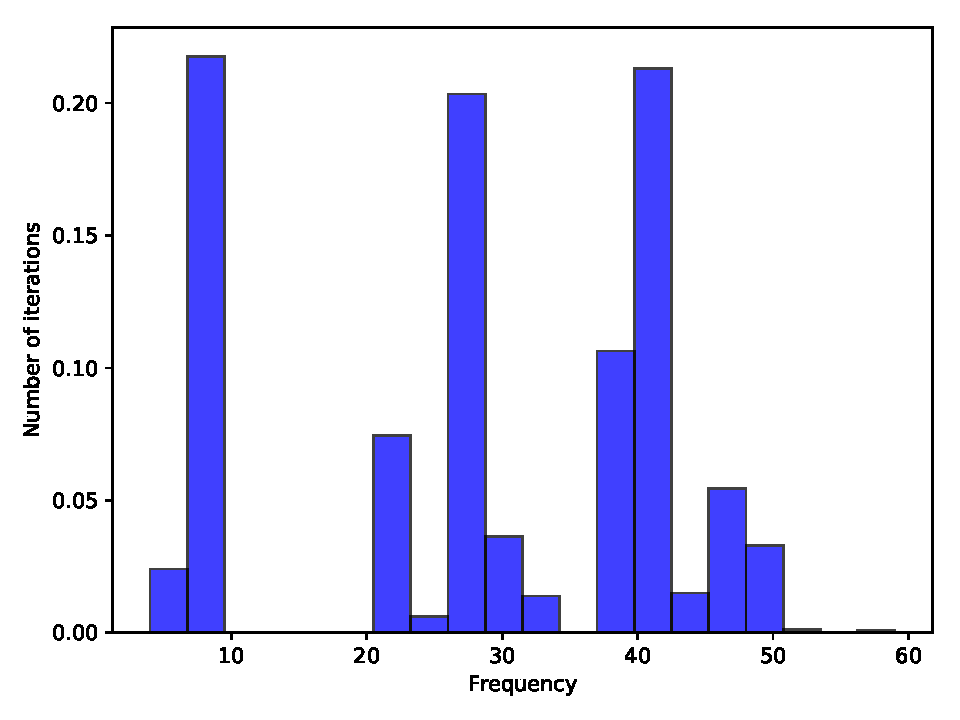
\includegraphics[width=\textwidth]{sphericalEM4_iterations_hist.pdf}
      \caption{Histogram of the number of iterations}\label{fig:sphericalEM4-iterations-hist}
    \end{subfigure}
    \quad
    \begin{subfigure}[t]{0.48\textwidth}
      \centering
      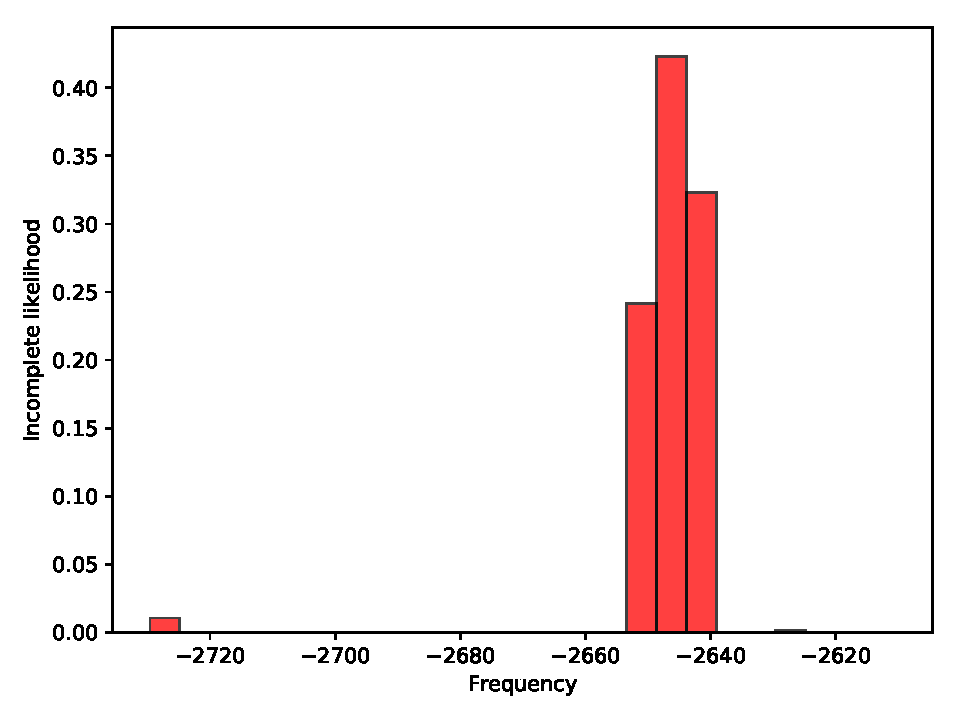
\includegraphics[width=\textwidth]{sphericalEM4_likelihood_hist.pdf}
      \caption{Histogram of the incomplete likelihood}\label{fig:sphericalEM4-distortion-hist}
    \end{subfigure}
    \caption{Histogram representing the number of iterations and the
      expected complete likelihood for $5000$ iterations of the
      spherical EM algorithm with $K=4$ and a tolerance of $10^{-4}$
      on the training data}\label{fig:sphericalEM4-hist}
  \end{figure}

  % Since for each $k \in \intn{1}{K}$, we have a diagonal covariance
  % matrix $\Sigma_k = \sigma_k^2 I$,
  % To represent the ellipses that contain a percentage of the
  % distribution, I use the $\chi^2$

  \begin{figure}[h!]
    \centering
    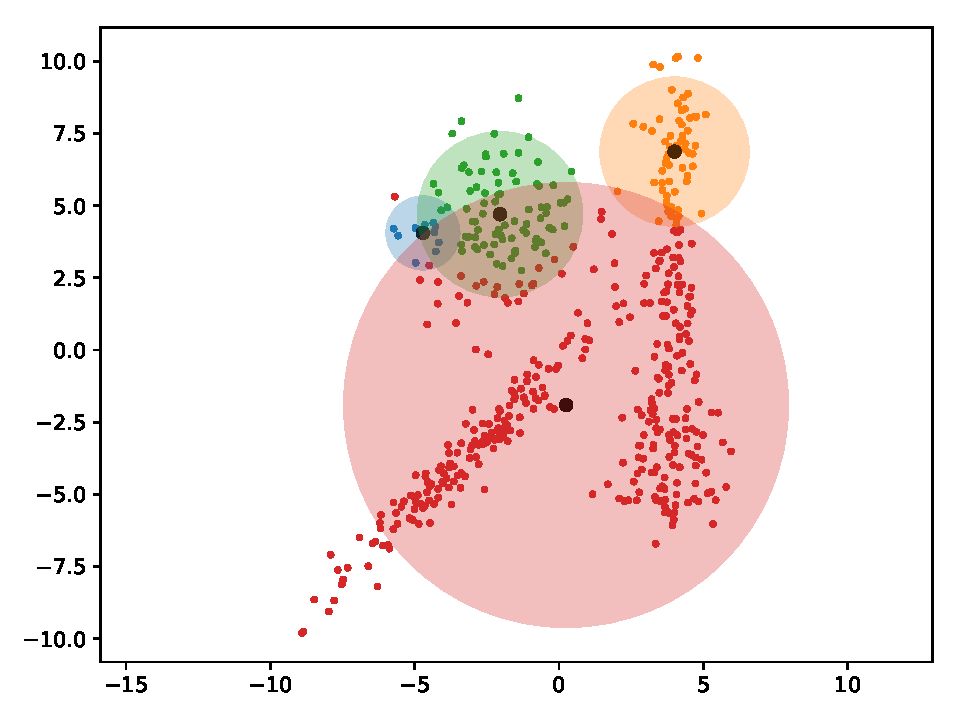
\includegraphics[width=0.7\textwidth]{sphericalEM4_failure.pdf}
    \caption{Representation of the training points, the means returned
      by an execution of the spherical EM algorithm ($K = 4$) that is
      stuck in a local minimum. the disks represented contain 90\% of
      the mass of the associated gaussian distribution (it fails to
      converge to the global minimum) (likelihood = -2727.57,
      convergence in 128 iterations, for
      $\epsilon = 10^{-6}$)}\label{fig:sphericalEM4-failure}
    % -2727.57347322
  \end{figure}

\end{subquestion}

\clearpage
\begin{subquestion}
  The result for an execution of the EM algorithm for gaussian mixture
  with general covariance is represented on figure
  \ref{fig:fullEM4-success}. As for the spherical case, each point of
  the training example is represented in the color of the most
  probable value of the corresponding latent variable. For each of the
  K gaussian distribution, the mean is represented in black, the
  ellipse containing $90\%$ of the distribution is also
  represented. The evolution of the incomplete log likelihood is
  represented in the figure \ref{fig:fullEM4-likelihood}.

  \begin{figure}[h!]
    \centering
    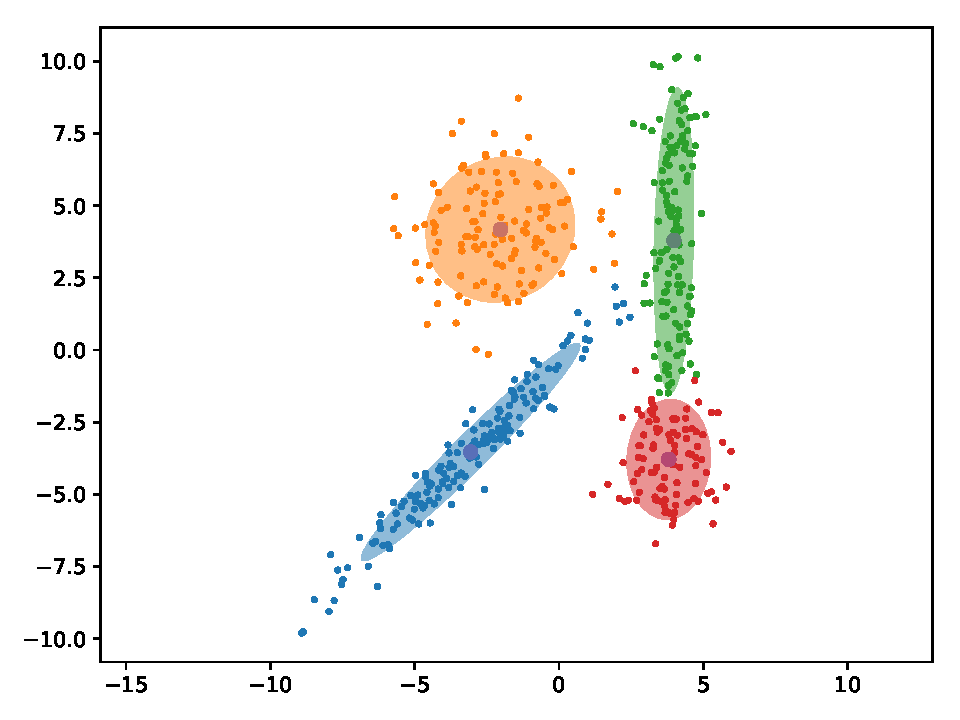
\includegraphics[width=0.7\textwidth]{fullEM4_success.pdf}
    \caption{Representation of the training points, the means returned
      by an execution of the full EM algorithm ($K = 4$). the
      disks represented contain 90\% of the mass of the associated
      gaussian distribution (likelihood = $-2327.72$, convergence in $26$
      iterations with $\epsilon = 10^{-6}$)}\label{fig:fullEM4-success}
    % incomplete likelihood -2327.71703039
  \end{figure}

  \begin{figure}[h!]
    \centering
    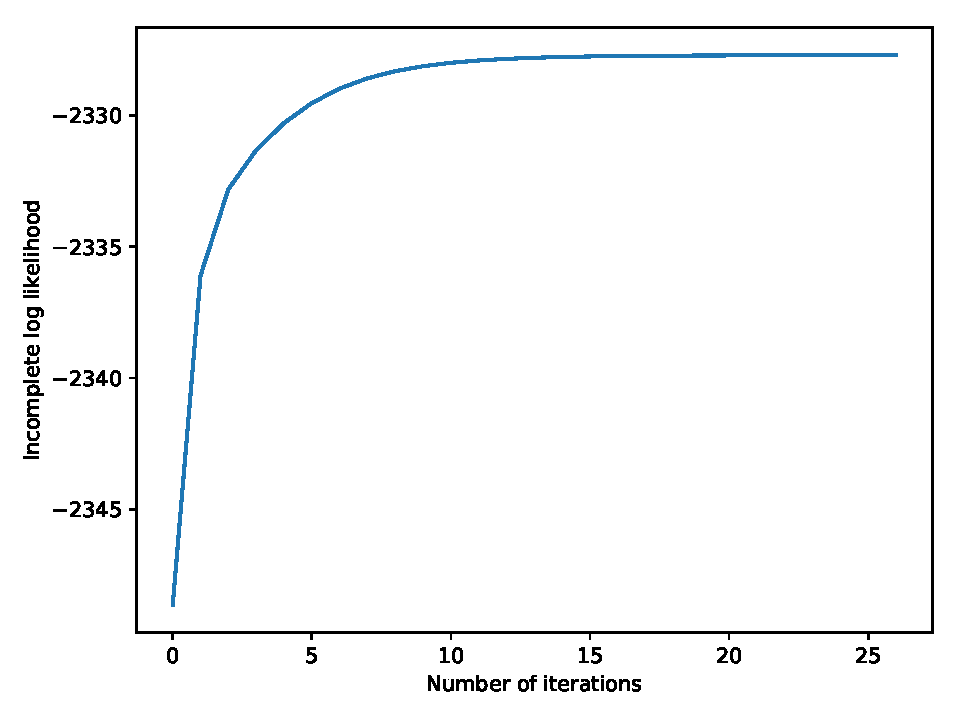
\includegraphics[width=0.6\textwidth]{fullEM4_likelihood.pdf}
    \caption{Evolution of the incomplete log likelihood with respect
      to the number of iterations for an execution of the EM algorithm
      for gaussian mixture with general covariance (converges a
      likelihood = $-2327.72$, in 26 iterations with
      $\epsilon = 10^{-6}$) }\label{fig:fullEM4-likelihood}
  \end{figure}


  I've also run $5000$ iteration of the algorithm on training sample,
  and plotted the histogram representing the number of iteration and
  the incomplete log likelihood it has converged to
  \figref{fig:fullEM4-hist}).  In the histogram, the estimated
  frequencies corresponding to each of the two bars are $1.42\%$ and
  $98.58\%$. The figure \ref{fig:fullEM4-failure} presents a case
  where the algorithm has converged to a different local minimum
  (corresponding to the first bar in the histogram).

  The algorithm has the same stopping criterion as in the spherical
  case.

  \begin{figure}[h!]
    \centering
    \begin{subfigure}[t]{0.48\textwidth}
      \centering
      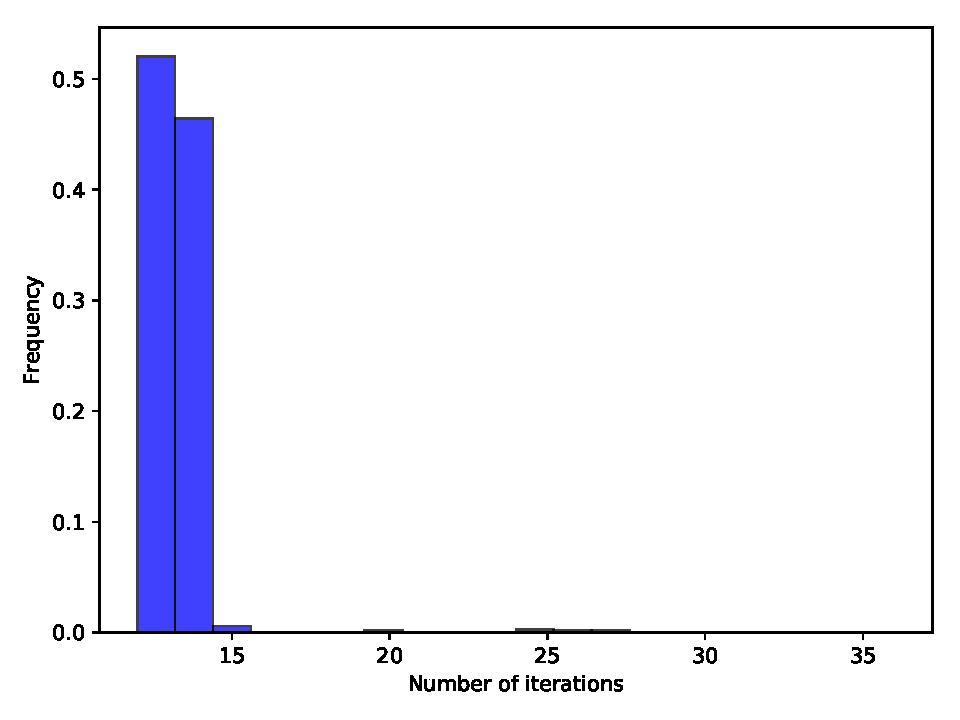
\includegraphics[width=\textwidth]{fullEM4_iterations_hist.pdf}
      \caption{Histogram of the number of iterations}\label{fig:fullEM4-iterations-hist}
    \end{subfigure}
    \quad
    \begin{subfigure}[t]{0.48\textwidth}
      \centering
      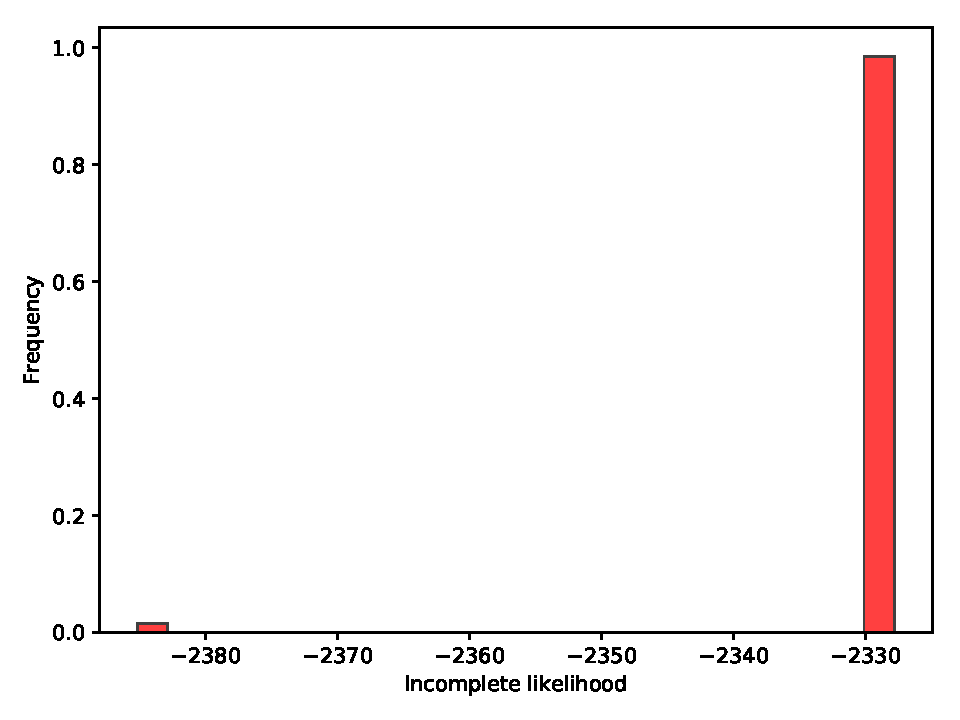
\includegraphics[width=\textwidth]{fullEM4_likelihood_hist.pdf}
      \caption{Histogram of the incomplete likelihood}\label{fig:fullEM4-distortion-hist}
    \end{subfigure}
    \caption{Histogram representing the number of iterations and the
      expected complete likelihood for $5000$ iterations of the
      full EM algorithm with $K=4$ and a tolerance of $10^{-4}$
      on the training data}\label{fig:fullEM4-hist}
  \end{figure}

  \begin{figure}[h!]
    \centering
    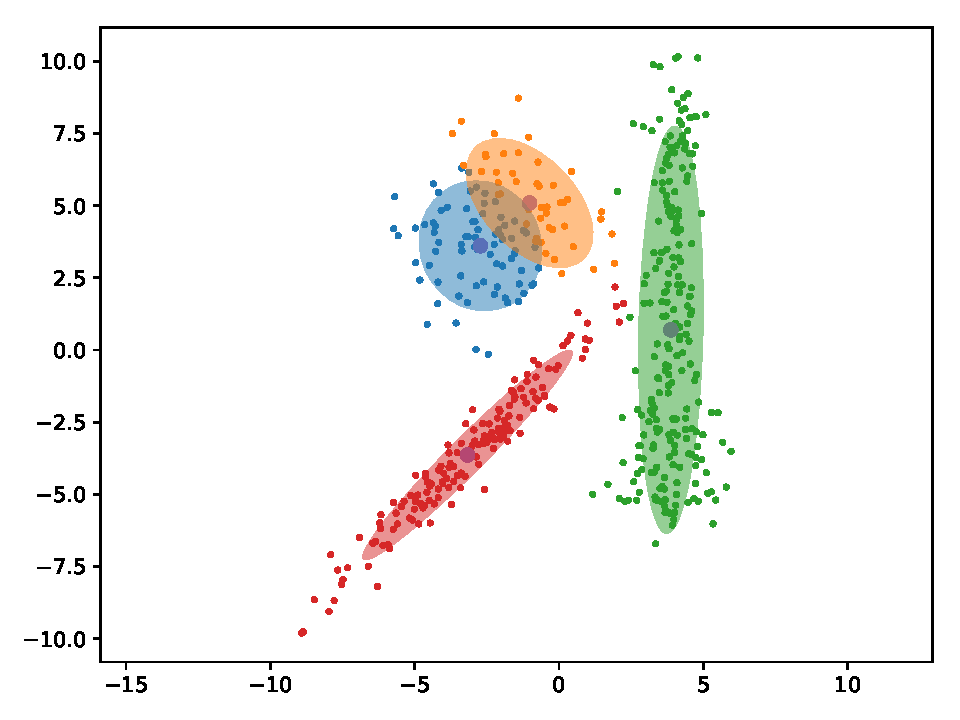
\includegraphics[width=0.7\textwidth]{fullEM4_failure.pdf}
    \caption{Representation of the training points, the means returned
      by an execution of the full EM algorithm ($K = 4$). the
      disks represented contain 90\% of the mass of the associated
      gaussian distribution (likelihood = -2383.64, convergence in 99
      iterations, with $\epsilon = 10^{-6}$)}\label{fig:fullEM4-failure}
    % incomplete likelihood -2383.63787383
  \end{figure}

\end{subquestion}

\begin{subquestion}
  I've trained each algorithm (Kmeans, EM for gaussian mixture model
  with isotropic and general covariance) $500$ times, for each train,
  I've measured the distortion / incomplete likelihood after training
  for both the training and the test data. The results are given in the
  table \ref{tab:comparison-distortion-likelihood}.

  \begin{table}[h!]
    \centering
    \begin{tabular}{| l | c | c || c | c |}
      \hline
      & \multicolumn{2}{c||}{\textbf{Train}} & \multicolumn{2}{c|}{\textbf{Test}} \\
      \hline
      \multicolumn{1}{|c|}{Method} & Mean & Std & Mean & Std \\
      \hline
      Kmeans (Distortion)            & 3382.60  & 891.92 & 3224.83  & 742.64  \\
      Kmeans++ (Distortion)          & 3293.13  & 355.21 & 3152.40  & 325.07  \\
      \hline
      EM Isotropic GMM (Likelihood)  & -2652.89 & 15.17  & -2654.39 & 23.01  \\
      EM General GMM (Likelihood)    & -2332.29 & 17.97 & -2417.30 & 19.77 \\
      \hline
    \end{tabular}
    \captionof{table}{Comparison of the mean and standard deviation of
      the distortion / likelihood between the train and test data
      (obtained for $500$ trains of the algorithm)} \label{tab:comparison-distortion-likelihood}
  \end{table}

  \newpage
  \ipart{Kmeans}

  The first thing to notice is that the Kmeans is not really adapted
  to cluster these king of data, the data has clearly been generated
  by a weighted sum of gaussian kernels of general covariances.

  We see that the standard deviation of the distortion provided by
  Kmeans is very large even though the mean is close from what we have
  observed as the best local minimum ($3237.78$), this shows that the
  Kmeans algorithm sometimes fails and get stuck in a \say{bad} local
  minimum, this agrees with what we have seen in the dedicated
  question (in particular with the histogram presented in figure
  \ref{fig:kmeans4-hist}), we have seen in this histogram that the
  algorithm behaved well $99.42\%$ of the time on $5000$ trains.  To
  have a good probability of getting a good behavior, we could restart
  the algorithm $N$ times and keep the best distortion. Then non
  formally, the probability of getting a \say{good} result will be
  $1 - (1 - p)^N$ where $p$ is the probability of having a \say{good}
  result.

  Despite the fact that it is not really adapted to the data, the
  output of Kmeans is quite consistent.


  \ipart{Isotropic vs general covariance}

  The EM algorithm for gaussian mixture with general covariance
  performs better than the one for gaussian mixture with isotropic
  covariance, this is not a surprise, because this model is more
  general than the other, and the data are particularly adapted to
  this model (they really seem to be generated by a weighted sum of
  gaussian kernels that do not have isotropic covariance matrix).
  Despite that, the EM for isotropic gaussian mixture has a
  low standard deviation, and also gives a consistent result (see the
  histogram in figure \ref{fig:sphericalEM4-hist}).

  We can see that in the case of the general covariance, the EM
  algorithm converges faster compared to the isotropic case. We can
  see in the histograms on figure \ref{fig:sphericalEM4-hist} and
  \ref{fig:fullEM4-hist}, and by comparing the evolution of the
  incomplete log likelihood for both cases
  (\ref{fig:sphericalEM4-likelihood} and
  \ref{fig:fullEM4-likelihood}), we see that in the general covariance
  case this fonction converges really fast,
  whereas in the isotropic case, the function goes through unstable
  points, which traduces that the maximization problem is less
  regular.

\end{subquestion}

\subsection*{Kmeans++}

I've also implemented Kmeans++, because I wanted to know how much
it would change the results. Unfortunately, I did not have time
to exploit the results. I've put the result of \emph{Kmeans++}
in the table \ref{tab:comparison-distortion-likelihood}, and
the figure \ref{fig:Kmeanspp} represents the different
steps for the initialization of the points with the algorithm,
the distances, and hence the probabilities of beeing chosen at
the next step, are represented in color scale for each point.

\begin{figure}[h!]
  \centering
  \begin{subfigure}[t]{0.48\textwidth}
    \centering
    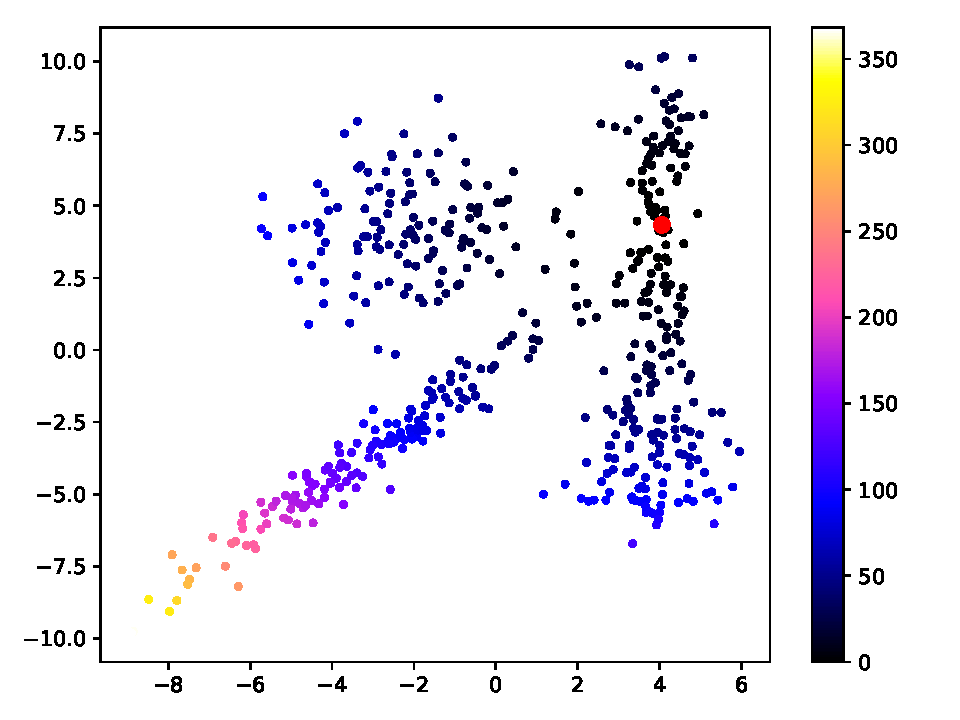
\includegraphics[width=\textwidth]{Kmeanspp_P0.pdf}
    \caption{First point chosen}\label{fig:Kmeanspp-p0}
  \end{subfigure}
  \quad
  \begin{subfigure}[t]{0.48\textwidth}
    \centering
    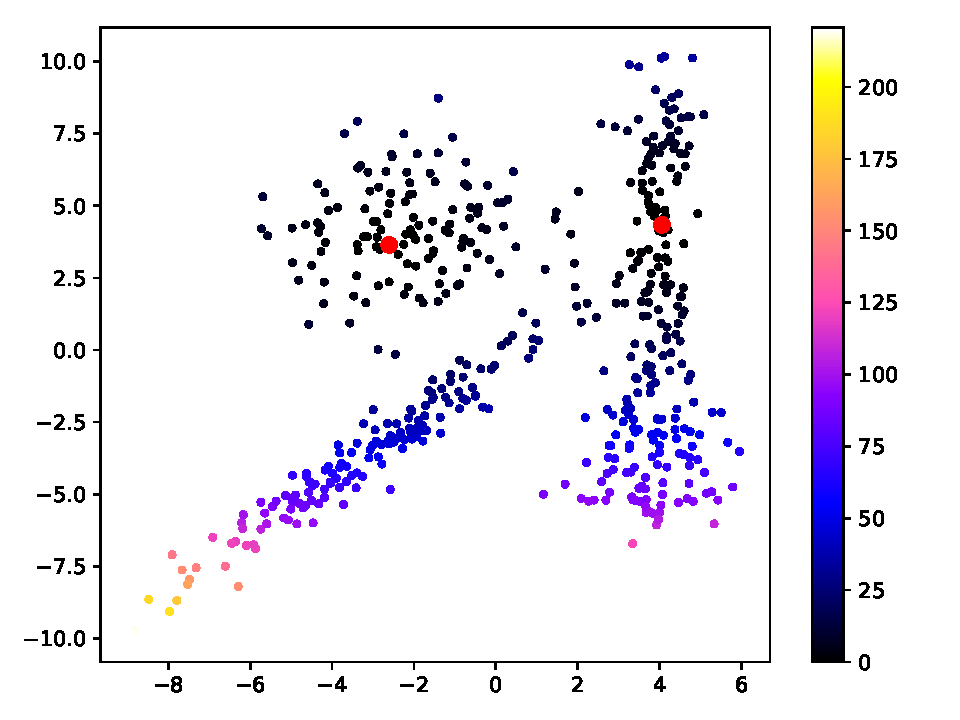
\includegraphics[width=\textwidth]{Kmeanspp_P1.pdf}
    \caption{Second point chosen}\label{fig:Kmeanspp-p1}
  \end{subfigure} \\
  \begin{subfigure}[t]{0.48\textwidth}
    \centering
    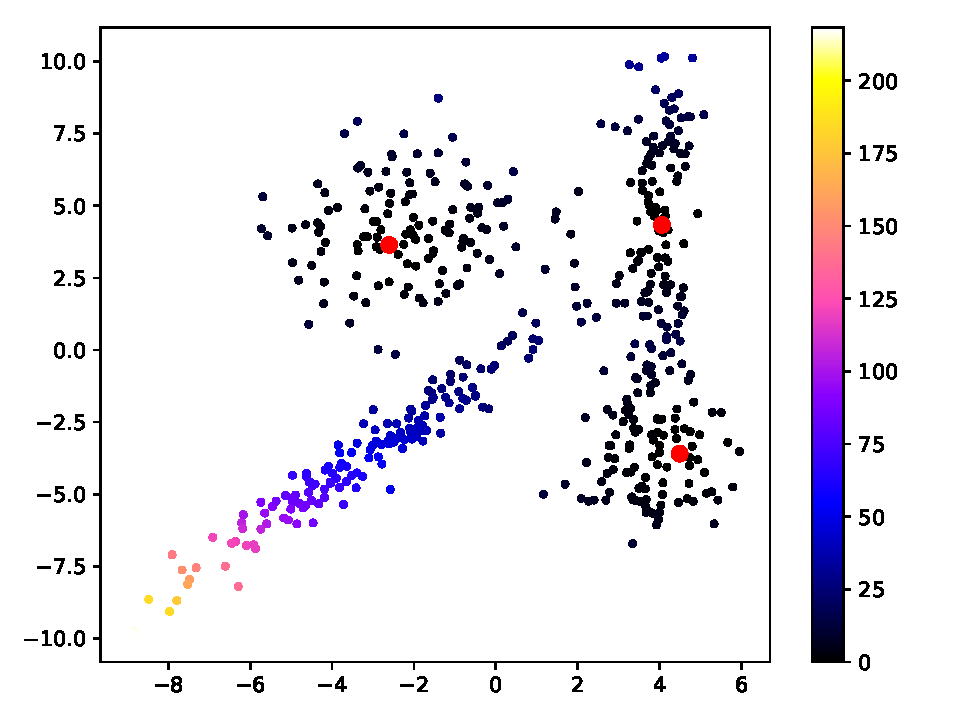
\includegraphics[width=\textwidth]{Kmeanspp_P2.pdf}
    \caption{Third point chosen}\label{fig:Kmeanspp-p2}
  \end{subfigure}
  \quad
  \begin{subfigure}[t]{0.48\textwidth}
    \centering
    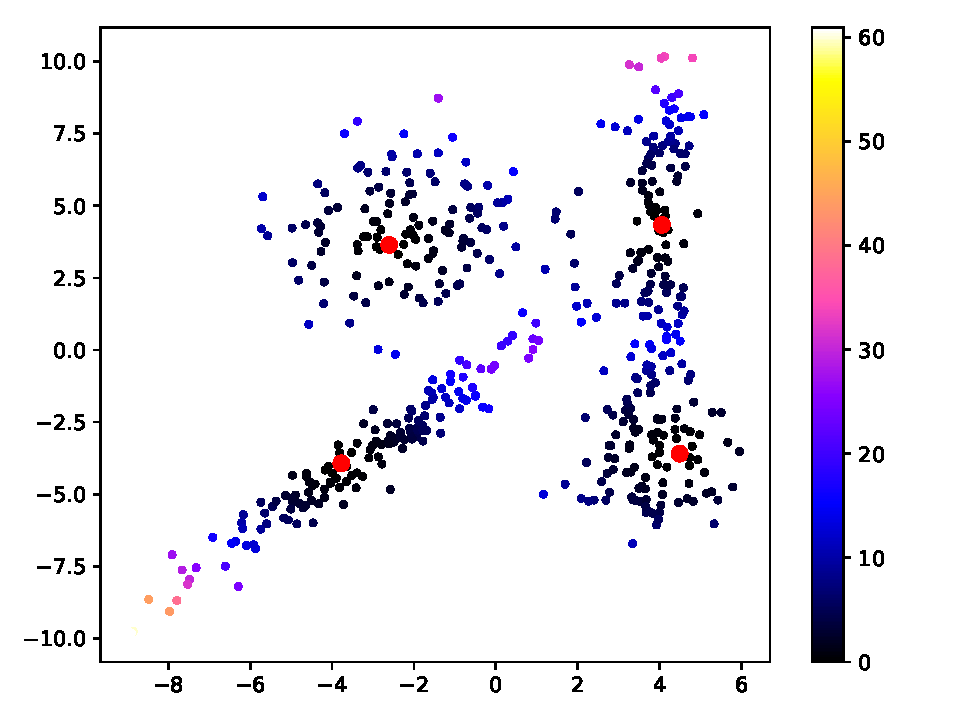
\includegraphics[width=\textwidth]{Kmeanspp_P3.pdf}
    \caption{Last point chosen}\label{fig:Kmeanspp-p3}
  \end{subfigure}
  \caption{Representation of the points chosen by the K-means++
    algorithm and probability of selecting points at each
    steps}\label{fig:Kmeanspp}
\end{figure}

\section{Conclusion}


I've spent a lot of time improving the code, it uses extensively the
numpy broadcasting mechanism and do computations on multidimensional
arrays to make the computation very efficient (there's basically no
loop). I've measured the performances to be more or less equivalent to
scikit-learn for the given data (It's about $10\%$ slower
\emph{scikit-learn} for the isotropic case and $10\%$ faster for the
general case, when tested on 500 runs of the training data for
$\epsilon = 10^{-6}$ on my matchine). I would have loved to optimize
more but it would have seriously impacted the readability of my code.

\section{Content of the archive}

\begin{itemize}
\item clustering.py : contains all the clustering method (Kmeans,
  Kmeans++, EM isotropic GMM, EM general GMM), this is the main class
  everything depends on.
\item comp\_likelihood.py : print the values of the distortion and likelihood
  for each methods (produces the table \ref{tab:comparison-distortion-likelihood})
\item comp\_scikit.py : compares the performances of my algorithm and
  \emph{scikit-learn}'s
\item kmeans.py run Kmeans algorithm and plots the result
\item spherical\_em.py : runs EM for gaussian mixture with isotropic
  covariance and plots the result
\item full\_em.py : runs EM for gaussian mixture with general
  covariance and plots the result
\item histograms.py : plots the histograms presented in the figures
  \ref{fig:kmeans4-hist}, \ref{fig:sphericalEM4-hist} and
  \ref{fig:fullEM4-hist}
\item likelihood.py : plots the distortion or likelihood w.r.t the
  number of iteration
\item voronoi.py : function found on the internet
  (https://gist.github.com/pv/8036995) to plot a voronoi graph given
  points.
\end{itemize}



%% \begin{figure}[p]
%%   \centering
%%   \begin{subfigure}[t]{0.40\textwidth}
%%     \centering
%%     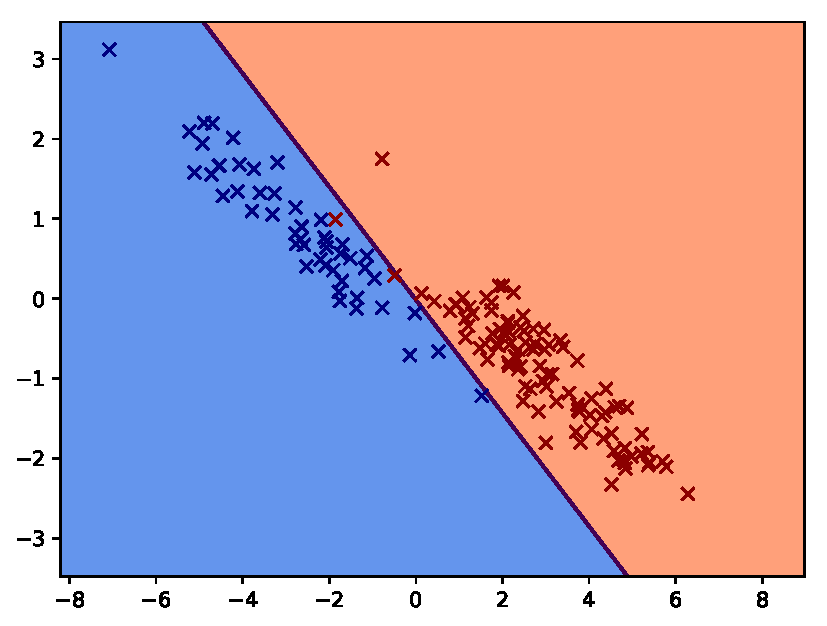
\includegraphics[width=\textwidth]{LDA_classificationA_train.pdf}
%%     \caption{Training observations A ($150$ points)}\label{fig:LDA-A-train}
%%   \end{subfigure}
%%   \quad
%%   \begin{subfigure}[t]{0.40\textwidth}
%%     \centering
%%     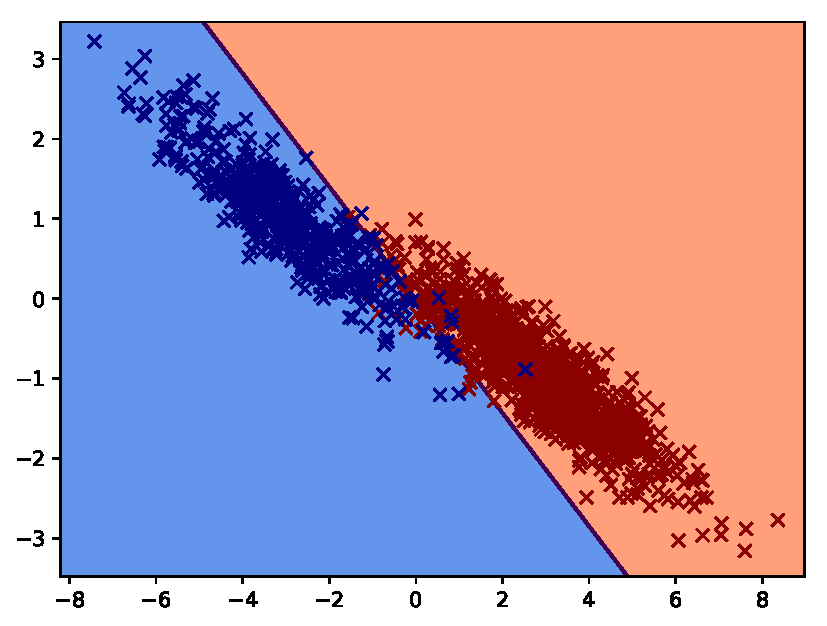
\includegraphics[width=\textwidth]{LDA_classificationA_test.pdf}
%%     \caption{Test observations A ($1500$ points)}\label{fig:LDA-A-test}
%%   \end{subfigure}
%%   \vskip\baselineskip
%%   \begin{subfigure}[t]{0.40\textwidth}
%%     \centering
%%     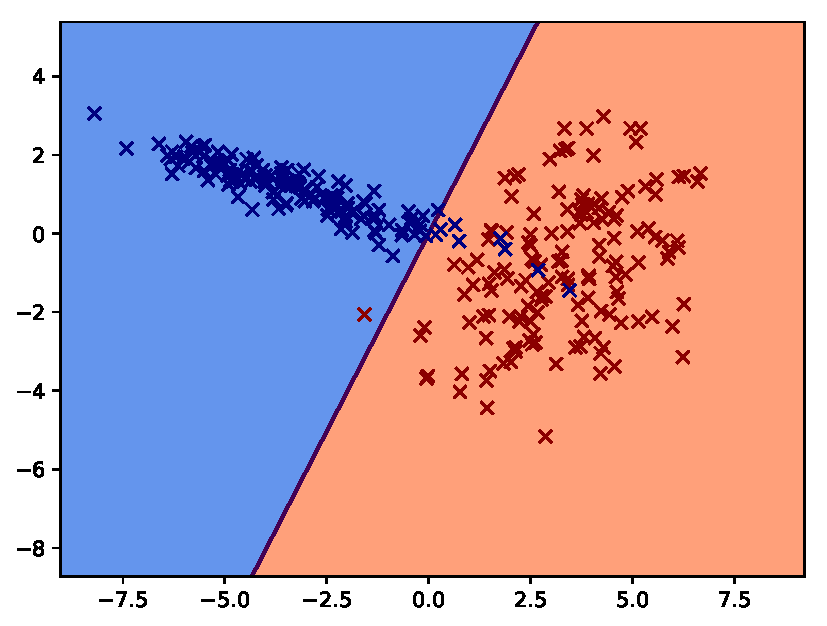
\includegraphics[width=\textwidth]{LDA_classificationB_train.pdf}
%%     \caption{Training observations B ($150$ points)}\label{fig:LDA-B-train}
%%   \end{subfigure}
%%   \quad
%%   \begin{subfigure}[t]{0.40\textwidth}
%%     \centering
%%     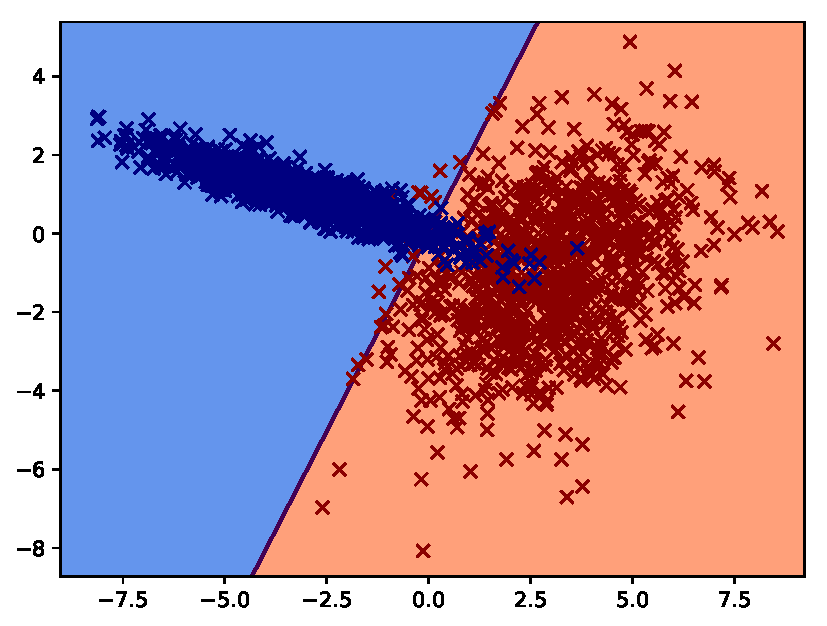
\includegraphics[width=\textwidth]{LDA_classificationB_test.pdf}
%%     \caption{Test observations B ($1500$ points)}\label{fig:LDA-B-test}
%%   \end{subfigure}
%%   \vskip\baselineskip
%%   \begin{subfigure}[t]{0.40\textwidth}
%%     \centering
%%     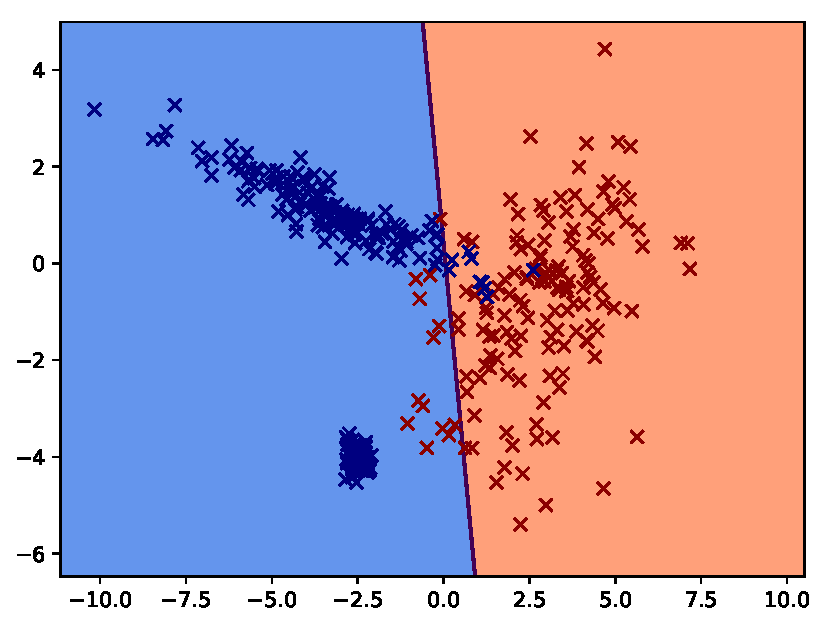
\includegraphics[width=\textwidth]{LDA_classificationC_train.pdf}
%%     \caption{Training observations C ($150$ points)}\label{fig:LDA-C-train}
%%   \end{subfigure}
%%   \quad
%%   \begin{subfigure}[t]{0.40\textwidth}
%%     \centering
%%     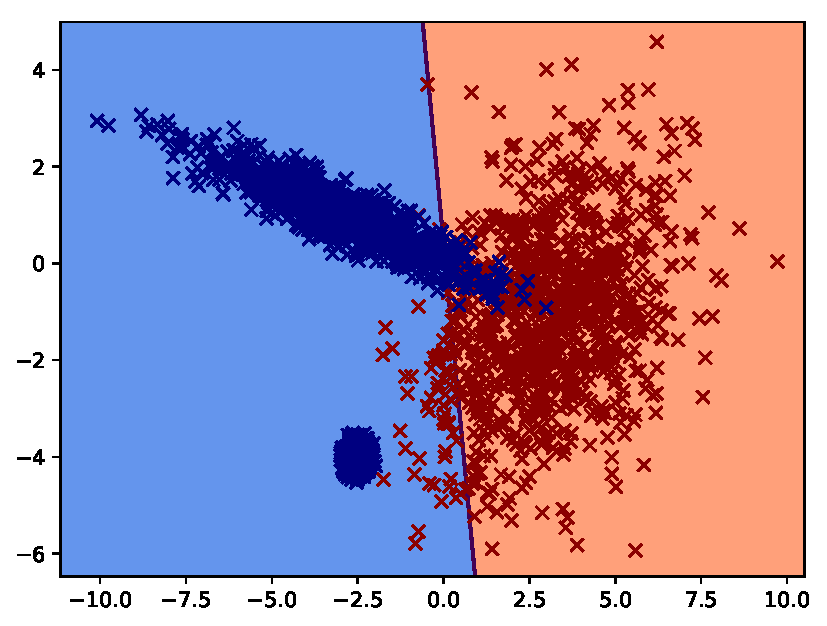
\includegraphics[width=\textwidth]{LDA_classificationC_test.pdf}
%%     \caption{Test observations C ($1500$ points)}\label{fig:LDA-C-test}
%%   \end{subfigure}
%%   \caption{Sample data and decision boundary representation for the LDA classifier on the three files}\label{fig:LDA}
%% \end{figure}


%% \begin{table}[h!]
%%   \centering
%%   \begin{tabular}{| l | l | l | l | c | c |}
%%     \hline
%%     sample file & $\pi$ & $\mu_0$ & $\mu_1$ & $\Sigma_0$ & $\Sigma_1$ \\
%%     \hline
%%     \file{classificationA} &
%%     0.33 & ( 2.90, -0.89 ) & ( -2.69, 0.87  ) &
%%     \( \left( \begin{array}{cc}
%%       2.33 & -1.06 \\
%%       -1.06 &  0.58
%%     \end{array} \right) \) &
%%     \( \left( \begin{array}{cc}
%%       2.76 & -1.33 \\
%%       -1.33 &  0.70 \\
%%     \end{array} \right) \) \\

%%     \file{classificationB} &
%%     0.5 & ( 3.34, -0.84 ) & ( -3.22, 1.08) &
%%     \( \left( \begin{array}{cc}
%%       2.56 &  1.07 \\
%%       1.07 &  2.98 \\
%%     \end{array} \right)  \) &
%%     \( \left( \begin{array}{cc}
%%       4.18 & -1.34 \\
%%       -1.34 &  0.52 \\
%%     \end{array} \right)  \) \\

%%     \file{classificationC} &
%%     0.625 & ( 2.79, -0.84 ) & ( -2.94,-0.96 ) &
%%     \( \left( \begin{array}{cc}
%%       2.92 &  1.25 \\
%%       1.25 &  2.94  \\
%%     \end{array} \right)  \) &
%%     \( \left( \begin{array}{cc}
%%       2.88 &  -1.77 \\
%%       -1.77 &  6.59 \\
%%     \end{array} \right)  \) \\
%%     \hline
%%   \end{tabular}
%%   \captionof{table}{Parameters learnt for the QDA method for the different training sample} \label{tab:ParamQDA}
%% \end{table}


\end{document}
